\documentclass[letterpaper,10pt]{book}
% Change to 10 pt
\usepackage{pdfpages}
\usepackage{morewrites}			% to counteract the no write space problem
\setcounter{tocdepth}{5}

\usepackage[framemethod=TikZ]{mdframed}

\usepackage{fancyhdr}

\usepackage{paralist}
\usepackage{amsmath}
\usepackage{amsfonts}
\usepackage{amssymb}
\usepackage{graphicx}

\usepackage{datetime}
%\usepackage{ulem}

%\usepackage[nottoc]{toobibind}

\usepackage[inline]{enumitem}

% Outer margin at 2.50 is exactly correct to fit the ``corruption alert'' tables
\usepackage[inner=1.0in, outer=2.50in, top=2.54cm,bottom=2.54cm, marginparwidth=2.25in]{geometry}

\usepackage{marginnote}
\usepackage{longtable}
\usepackage{booktabs}
\usepackage{xcolor}

\usepackage{soul}

\usepackage{marginnote}
\usepackage{imakeidx} 
\usepackage[
	backref=true,
	style=numeric,
%	citestyle=numeric,
	backend=bibtex
	]{biblatex}
\usepackage[driverfallback=hypertex,colorlinks=True]{hyperref}
\usepackage{cleveref}

\makeindex[name=scripture,columnsep=20pt, columnseprule=True,columns=3, title=Scripture References]
\makeindex[name=speaker,columnsep=20pt, columnseprule=True,,columns=2, title=Sermon Creator]
\makeindex[name=series,columnsep=20pt, columnseprule=True,,columns=2, title=Sermon Series]
\makeindex[name=date,columnsep=20pt, columnseprule=True,columns=2, title=Sermon Date]

\makeindex[name=event,columnsep=20pt, columnseprule=True,columns=2, title=Event]

\makeindex[name=topic,columnsep=20pt, columnseprule=True,columns=2, title=Topic]
\makeindex[name=AWIP,columnsep=20pt, columnseprule=True,columns=3, title=All Words in Passage]
\makeindex[name=NWIV,columnsep=20pt, columnseprule=True,columns=3, title=Number of Words in Verse]
\makeindex[name=PNIP,columnsep=20pt, columnseprule=True,columns=3, title=Proper Names in Passage]
\makeindex[name=PEIP,columnsep=20pt, columnseprule=True,columns=2, title=Prophetic Events in Passage]


\makeindex[name=TWPAQ,columnsep=20pt, columnseprule=True,columns=1, title=13-Word Phrases and Quotes]
\makeindex[name=PFTTIS,columnsep=20pt, columnseprule=False,columns=3, title=Phrases found 13 times in scripture]
\makeindex[name=WFTTIS,columnsep=20pt, columnseprule=False,columns=3, title=Words found 13 times in scripture]
\makeindex[name=WFITV,columnsep=20pt, columnseprule=False,columns=3, title=Words found in exactly 13 verses]
\makeindex[name=EVENTS,columnsep=20pt, columnseprule=False,columns=2, title=Sermon Log by Place]
\makeindex[name=QUESTIONS,columnsep=20pt, columnseprule=False,columns=2, title=Bible Questions]

\makeindex[name=DOCTRINES,columnsep=20pt, columnseprule=False,columns=2, title=Doctrines]

\makeindex[name=SONGS,columnsep=20pt, columnseprule=False,columns=1, title=Songs]
\makeindex[name=LOCATION,columnsep=20pt, columnseprule=False,columns= 2, title=Location]
\makeindex[name=FACEBOOK,columnsep=20pt, columnseprule=False,columns=2, title=Facebook]

\makeindex[name=DEVOTIONAL,columnsep=20pt, columnseprule=False,columns=1, title=Devotionals]

\pagestyle{fancy}
\fancyhf{}
\fancyhead[LE,RO]{\today}
\fancyhead[RE,LO]{Notes, Outlines, Comments}
\fancyhead[CE,CO]{-page \thepage  - }

\fancyfoot[CO,CE]{\leftmark}
%\fancyfoot[LE,RO]{CSCE 692, HW1}

\title{DBR\\
Daily \\ Reads}
\author{Keith Anthony \\
\today }
%\title

%+/ffffff +   \pagenumbering{gobble}

\bibliography{Bibliographies/All20220108}

%%%%% TWEAKS:
%%% - distance from fcolorbox frame to text
\setlength{\fboxsep}{1.0pt}

\usepackage[utf8]{inputenc}
\usepackage{tikz}

%%%%%%%%%%%%%%%%%%%%%%%%%%%%%%%%%%%%%%%%%%%%%%%%%%%%%%%%%%%%%%%%%%%%%%%%%%%%%%%%

\begin{document}

\begin{titlepage}

% Set the text of the page to right-aligned until \end{flushright}
\begin{flushright}
\rightskip=-2.5cm

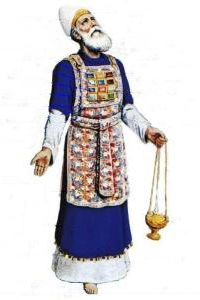
\includegraphics[width=50mm,scale=1.5]{Melchisedec.jpg}
\vspace{0.4in}

% Create a title for the document and write it in bold font
\LARGE{\textbf{\date}}
\linebreak

\vspace{0.5in}


\begin{flushleft}
\LARGE{Job\\}\vspace{0.25in}
\LARGE{Notes, Outlines, Comments}
\end{flushleft}

% write in large letters
%\large{Free webservices and apps}

% Skip some space
\vspace{0.6in}

%\large{Documentation}
% Skip some space

\bigskip

\normalsize{Xenia, Oh.\\}
\normalsize{created: \today}

% Skip some space
\vspace{1.3in}

\end{flushright}
% End the title page
\end{titlepage}

%\titlehttps://www.overleaf.com/project/60d732302fc633866943c9d2JE

\newpage 

\tableofcontents\hypertarget{TOC}{}
\listoffigures
\listoftables

\hyphenation{A-bim-e-lech bre-thren E-phra-im  Gib-e-o-nites Jer-u-sa-lem through-out Phil-i-stines The-o-phil-us Am-a-le-kites ven-geance Mesh-el-e-mi-ah onan-ism Phar-a-oh Py-thon thoughts grev-ous-ness Hach-a-liah adul-ter-er Shad-rach}

%\fcolorbox{black}{bone}{TEXT}
%%%%%%%%%%%%%%%%% EXTRA COLORS
%%%%%%%%%%%%%%%%% EXTRA COLORS
%%%%%%%%%%%%%%%%% EXTRA COLORS
\definecolor{champagne}{rgb}{0.97,0.91,0.81}
\definecolor{bone}{rgb}{0.89,0.85,0.79}

\definecolor{ForestGreen}{rgb}{0.00,0.29,0.098}
\definecolor{GIVING}{cmyk}{1,0.0,0.72,.1}

\definecolor{MLPE}{cmyk}{1,1,0,.45}
\definecolor{SOCCER}{cmyk}{.77, 0, .42, .49}
\definecolor{PAYBILL}{cmyk}{0,0.83,0.76,0.07}
\definecolor{SERMON}{cmyk}{.14,.9,0,.30} % aka seance \href{http://www.flatuicolorpicker.com/purple-cmyk-color-model/}{seance}
\definecolor{BIBLE}{cmyk}{0,.17,.74,.17}
\definecolor{WORKBLUE}{cmyk}{1, .5, 0, .6}
\definecolor{myOrange}{cmyk}{0, .4, .98, .03}
\definecolor{myTan}{cmyk}{0.0,.07,.17,.10}
\definecolor{myRed}{cmyk}{0,1,1,0}
\definecolor{myWhite}{cmyk}{0,0,0,0}
\definecolor{BLUESoD}{cmyk}{.97,.84,0,.04}
\definecolor{WHITE}{cmyk}{0,0,0,0}
\definecolor{OLDGOLD}{cmyk}{0.05,0.3,1.00,0}
\definecolor{CASTLETON}{cmyk}{1,0,0.31,0.66}
\definecolor{cadmiumgreen}{rgb}{0.0, 0.42, 0.24}
\definecolor{jungle}{rgb}{0.203,0.4882,0.1718}
\definecolor{MYGOLD}{rgb}{1,.84,0}

\definecolor{MYLIGHTGRAY}{rgb}{.85,.85,.85}

\definecolor{codegreen}{rgb}{0,0.6,0}
\definecolor{codegray}{rgb}{0.5,0.5,0.5}
\definecolor{codepurple}{rgb}{0.58,0,0.82}
\definecolor{backcolour}{rgb}{0.95,0.95,0.92}



\mdfdefinestyle{MyFrame}{%
    linecolor=blue,
    outerlinewidth=2pt,
    roundcorner=5pt,
    innertopmargin=\baselineskip,
    innerbottommargin=\baselineskip,
    innerrightmargin=10pt,
    innerleftmargin=10pt,
    backgroundcolor=gray!25!white}


\mdfdefinestyle{MyFrame2}{%
    linecolor=black,
    outerlinewidth=2pt,
    roundcorner=5pt,
    innertopmargin=\baselineskip,
    innerbottommargin=\baselineskip,
    innerrightmargin=10pt,
    innerleftmargin=10pt,
    backgroundcolor=yellow!25!white}



%\input{PFTTIS}
%\input{WFTTIS}
%\input{WFITV}


\chapter{Job 1}

\begin{figure}
  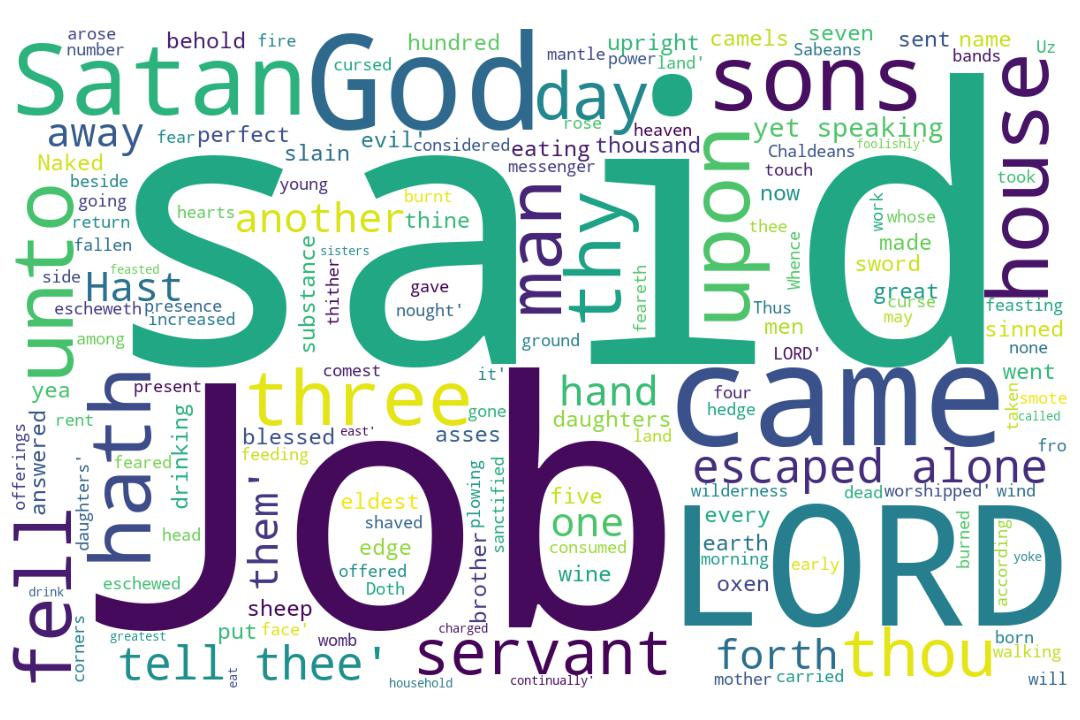
\includegraphics[width=\linewidth]{18OT-Job/Job1-WordCloud.jpg}
  \caption{Job 1 Word Cloud}
  \label{fig:Job 1 word Cloud}
\end{figure}


\marginpar{\scriptsize \centering \fcolorbox{black}{lime}{\textbf{WHY RIGHTEOUS SUFFER?}}\\ (Job 1:1-22) \begin{compactenum}[I.][8]
    \item  \textbf{To Prove a Point} \index[scripture]{Job!Job 01:08}(Job 1:8)
    \item  \textbf{To Purify} \index[scripture]{Job!Job 23:10}(Job 23:10, \index[scripture]{Psalms!Psa 17:03}Psa 17:3, \index[scripture]{1 Peter!1Pet 01:07}1Pet 1:7)
    \item \textbf{To make God Precious}
    \item \textbf{To Build Empathy} \index[scripture]{2 Corinthians!2Cor 1:2}(2Cor 1:4)
    \item \textbf{To Point out Self-Righteousness}
    \item Job \textbf{Pictures} Israel
    \item The Book \textbf{Portrays} the Tribulation
\end{compactenum}}


\marginpar{\scriptsize \centering \fcolorbox{black}{yellow}{\textbf{THE EXPERIMENT}}\\ (Job 1:6-12) \begin{compactenum}[I.][8]
    \item  The \textbf{Presentation} \index[scripture]{Job!Job 01:06}(Job 1:6)
    \item  A \textbf{Perfect} Man \index[scripture]{Job!Job 01:08}(Job 1:8)
    \item  The \textbf{Postulate} \index[scripture]{Job!Job 01:10}(Job 1:10)
    \item  A \textbf{Proposal} \index[scripture]{Job!Job 01:11}(Job 1:11)
    \item  The \textbf{Power} \index[scripture]{Job!Job 01:12}(Job 1:12)
    \item  A \textbf{Prohibition} \index[scripture]{Job!Job 01:12}(Job 1:12)
    \item  The \textbf{Presence} \index[scripture]{Job!Job 01:12}(Job 1:12)
\end{compactenum}}

\marginpar{\scriptsize \centering \textbf{\fcolorbox{black}{black}{\textcolor[cmyk]{0,0,0,0}{SETTING UP THE TEST}}}\\ (Job 1) \begin{compactenum}[I.][6]
    \item The \textbf{Angels} \index[scripture]{Job!Job 01:06} (Job 1:6) 
    \item An \textbf{Assembly} \index[scripture]{Job!Job 01:06} (Job 1:6) 
    \item The \textbf{Aversary} \index[scripture]{Job!Job 01:07} (Job 1:7) 
    \item The \textbf{Archetype} \index[scripture]{Job!Job 01:08} (Job 1:8) 
    \item An \textbf{Accusation} \index[scripture]{Job!Job 01:11} (Job 1:11) 
    \item The \textbf{Agreement} \index[scripture]{Job!Job 01:12} (Job 1:12) 
\end{compactenum}}

\footnote{\textcolor[cmyk]{0.99998,1,0,0}{\hyperlink{TOC}{Return to end of Table of Contents.}}}\footnote{\href{https://www.audioverse.org/english/audiobibles/books/ENGKJV/O/Job/1}{\textcolor[cmyk]{0.99998,1,0,0}{Job  Audio}}}\textcolor[cmyk]{0.99998,1,0,0}{There was a man in the land of Uz, whose name \emph{was} Job; and that man was perfect and upright, and one that feared God, and eschewed evil.}
[2] \textcolor[cmyk]{0.99998,1,0,0}{And there were born unto him seven sons and three daughters.}
[3] \textcolor[cmyk]{0.99998,1,0,0}{His substance also was seven thousand sheep, and three thousand camels, and five hundred yoke of oxen, and five hundred she asses, and a very great household; so that this man was the greatest of all the men of the east.}
[4] \textcolor[cmyk]{0.99998,1,0,0}{And his sons went and feasted \emph{in} \emph{their} houses, every one his day; and sent and called for their three sisters to eat and to drink with them.}
[5] \textcolor[cmyk]{0.99998,1,0,0}{And it was so, when the days of \emph{their} feasting were gone about, that Job sent and sanctified them, and rose up early in the morning, and offered burnt offerings \emph{according} to the number of them all: for Job said, It may be that my sons have sinned, and cursed God in their hearts. Thus did Job continually.}\\
\\
\P \textcolor[cmyk]{0.99998,1,0,0}{Now there was a day when the sons of God came to present themselves before the LORD, and Satan came also among them.}
[7] \textcolor[cmyk]{0.99998,1,0,0}{And the LORD said unto Satan, Whence comest thou? Then Satan answered the LORD, and said, From going to and fro in the earth, and from walking up and down in it.}
[8] \textcolor[cmyk]{0.99998,1,0,0}{And the LORD said unto Satan, Hast thou considered my servant Job, that \emph{there} \emph{is} none like him in the earth, a perfect and an upright man, one that feareth God, and escheweth evil?}
[9] \textcolor[cmyk]{0.99998,1,0,0}{Then Satan answered the LORD, and said, Doth Job fear God for nought?}
[10] \textcolor[cmyk]{0.99998,1,0,0}{Hast not thou made an hedge about him, and about his house, and about all that he hath on every side? thou hast blessed the work of his hands, and his substance is increased in the land.}
[11] \textcolor[cmyk]{0.99998,1,0,0}{But put forth thine hand now, and touch all that he hath, and he will curse thee to thy face.}
[12] \textcolor[cmyk]{0.99998,1,0,0}{And the LORD said unto Satan, Behold, all that he hath \emph{is} in thy power; only upon himself put not forth thine hand. So Satan went forth from the presence of the LORD.}\\
\\
\P \textcolor[cmyk]{0.99998,1,0,0}{And there was a day when his sons and his daughters \emph{were} eating and drinking wine in their eldest brother's house:}
[14] \textcolor[cmyk]{0.99998,1,0,0}{And there came a messenger unto Job, and said, The oxen were plowing, and the asses feeding beside them:}
[15] \textcolor[cmyk]{0.99998,1,0,0}{And the Sabeans fell \emph{upon} \emph{them}, and took them away; yea, they have slain the servants with the edge of the sword; and I only am escaped alone to tell thee.}
[16] \textcolor[cmyk]{0.99998,1,0,0}{While he \emph{was} yet speaking, there came also another, and said, The fire of God is fallen from heaven, and hath burned up the sheep, and the servants, and consumed them; and I only am escaped alone to tell thee.}
[17] \textcolor[cmyk]{0.99998,1,0,0}{While he \emph{was} yet speaking, there came also another, and said, The Chaldeans made out three bands, and fell upon the camels, and have carried them away, yea, and slain the servants with the edge of the sword; and I only am escaped alone to tell thee.}
[18] \textcolor[cmyk]{0.99998,1,0,0}{While he \emph{was} yet speaking, there came also another, and said, Thy sons and thy daughters \emph{were} eating and drinking wine in their eldest brother's house:}
[19] \textcolor[cmyk]{0.99998,1,0,0}{And, behold, there came a great wind from the wilderness, and smote the four corners of the house, and it fell upon the young men, and they are dead; and I only am escaped alone to tell thee.}
[20] \textcolor[cmyk]{0.99998,1,0,0}{Then Job arose, and rent his mantle, and shaved his head, and fell down upon the ground, and worshipped,}
[21] \textcolor[cmyk]{0.99998,1,0,0}{And said, Naked came I out of my mother's womb, and naked shall I return thither: the LORD gave, and the LORD hath taken away; blessed be the name of the LORD.}
[22] \textcolor[cmyk]{0.99998,1,0,0}{In all this Job sinned not, nor charged God foolishly.}
\section{Job 1 Comments}

\subsection{Job 1:1}

\subsection{Job 1:2}

\subsection{Job 1:3}

\subsection{Job 1:4}

\subsection{Job 1:5}

\subsection{Job 1:6}
First real book ever written ?

Sons of God ... who are they? Not the godly line of Seth ... introduced to the chief character in scripture outside the lord ... 

Zech 3:1-2 second only to the godhead in wisdom and power ... one person in the Godhead rebuking with the authority of another
Ezek 28:3
Jude 9
Rev 12:9 power to deceive the whole world

At odds with the one system in the world that claims to be the true church
2 Cor 4:4
Eph 2:2 w Ezek 28:2 dan 11
10
2 Cor 11:14
King job 41:34
White horse rev 6:2 
Mt 4 quotes scripture
Rev 17:5 has a bride that is also a church also a city
Ministers 2 Cor 11:13
Own angels .. rev 13:14-18 ... devil and his angels
Cherub ... dragon .... man ... adversary
Rev 12:10-11

Here, it is devil as the accuser, 
appears in heaven with a company of angels
Pre-Adamic job 38:7 ... gods ... ps 82:1, 6 ... Genesis 3:5 ... some have defected and more will ... why?  \footnote{Michael Thomas, 04 December 2020, Job Lesson number 3.}

\subsection{Job 1:7}
Matt 26:50
Wherefore? Why are you here? the 

To and fro ... Zech 1:10\footnote{Michael Thomas, 04 December 2020, Job Lesson number 3.}

\subsection{Job 1:8}
In the earth ... 
see Acts 14:12 ... Jupiter and mercurial ... Jupiter vv 12, 13, 
Acts 19:15 ... black stone of Mecca ... kiss the black stone ... obelisk / monolith ... Rome ... Washington DC ... 2001 movie ... 

Perfect == mature, steadfast,\footnote{Michael Thomas, 04 December 2020, Job Lesson number 3.}

\subsection{Job 1:9}
Yes .... he knows all about him .... 
13 words in verse!\footnote{Michael Thomas, 04 December 2020, Job Lesson number 3.}

\subsection{Job 1:10}
1 Peter 5:8

Devil infers that if wealth and security were taken away, Job would fold
Satan saying, if you change his environment, things would be different!\footnote{Michael Thomas, 04 December 2020, Job Lesson number 3.}

\subsection{Job 1:11}
Exo 12:12 23 the Destroyer ... 1 Cor 10:10 ... rev 9:11 ...

Alleged contradiction: the Lord moved David ... 2 Sam 24:1 1 Chron 21:1 ... \footnote{Michael Thomas, 04 December 2020, Job Lesson number 3.}



\subsection{Job 1:12}

\subsection{Job 1:13}

\subsection{Job 1:14}

\subsection{Job 1:15}

\subsection{Job 1:16}

\subsection{Job 1:17}

\subsection{Job 1:18}

\subsection{Job 1:19}

\subsection{Job 1:20}

\subsection{Job 1:21}

\subsection{Job 1:22}



\index[NWIV]{28!Job!Job 1:1}\index[AWIP]{There!Job!Job 1:1}\index[AWIP]{was!Job!Job 1:1}\index[AWIP]{was!Job!Job 1:1 (2)}\index[AWIP]{a!Job!Job 1:1}\index[AWIP]{man!Job!Job 1:1}\index[AWIP]{man!Job!Job 1:1 (2)}\index[AWIP]{in!Job!Job 1:1}\index[AWIP]{the!Job!Job 1:1}\index[AWIP]{land!Job!Job 1:1}\index[AWIP]{of!Job!Job 1:1}\index[AWIP]{Uz!Job!Job 1:1}\index[AWIP]{whose!Job!Job 1:1}\index[AWIP]{name!Job!Job 1:1}\index[AWIP]{\emph{was}!Job!Job 1:1}\index[AWIP]{Job!Job!Job 1:1}\index[AWIP]{and!Job!Job 1:1}\index[AWIP]{and!Job!Job 1:1 (2)}\index[AWIP]{and!Job!Job 1:1 (3)}\index[AWIP]{and!Job!Job 1:1 (4)}\index[AWIP]{that!Job!Job 1:1}\index[AWIP]{that!Job!Job 1:1 (2)}\index[AWIP]{perfect!Job!Job 1:1}\index[AWIP]{upright!Job!Job 1:1}\index[AWIP]{one!Job!Job 1:1}\index[AWIP]{feared!Job!Job 1:1}\index[AWIP]{God!Job!Job 1:1}\index[AWIP]{eschewed!Job!Job 1:1}\index[AWIP]{evil!Job!Job 1:1}\index[AWIP]{\emph{was}!Job!Job 1:1}

\index[NWIV]{11!Job!Job 1:2}\index[AWIP]{And!Job!Job 1:2}\index[AWIP]{there!Job!Job 1:2}\index[AWIP]{were!Job!Job 1:2}\index[AWIP]{born!Job!Job 1:2}\index[AWIP]{unto!Job!Job 1:2}\index[AWIP]{him!Job!Job 1:2}\index[AWIP]{seven!Job!Job 1:2}\index[AWIP]{sons!Job!Job 1:2}\index[AWIP]{and!Job!Job 1:2}\index[AWIP]{three!Job!Job 1:2}\index[AWIP]{daughters!Job!Job 1:2}

\index[NWIV]{41!Job!Job 1:3}\index[AWIP]{His!Job!Job 1:3}\index[AWIP]{substance!Job!Job 1:3}\index[AWIP]{also!Job!Job 1:3}\index[AWIP]{was!Job!Job 1:3}\index[AWIP]{was!Job!Job 1:3 (2)}\index[AWIP]{seven!Job!Job 1:3}\index[AWIP]{thousand!Job!Job 1:3}\index[AWIP]{thousand!Job!Job 1:3 (2)}\index[AWIP]{sheep!Job!Job 1:3}\index[AWIP]{and!Job!Job 1:3}\index[AWIP]{and!Job!Job 1:3 (2)}\index[AWIP]{and!Job!Job 1:3 (3)}\index[AWIP]{and!Job!Job 1:3 (4)}\index[AWIP]{three!Job!Job 1:3}\index[AWIP]{camels!Job!Job 1:3}\index[AWIP]{five!Job!Job 1:3}\index[AWIP]{five!Job!Job 1:3 (2)}\index[AWIP]{hundred!Job!Job 1:3}\index[AWIP]{hundred!Job!Job 1:3 (2)}\index[AWIP]{yoke!Job!Job 1:3}\index[AWIP]{of!Job!Job 1:3}\index[AWIP]{of!Job!Job 1:3 (2)}\index[AWIP]{of!Job!Job 1:3 (3)}\index[AWIP]{oxen!Job!Job 1:3}\index[AWIP]{she!Job!Job 1:3}\index[AWIP]{asses!Job!Job 1:3}\index[AWIP]{a!Job!Job 1:3}\index[AWIP]{very!Job!Job 1:3}\index[AWIP]{great!Job!Job 1:3}\index[AWIP]{household!Job!Job 1:3}\index[AWIP]{so!Job!Job 1:3}\index[AWIP]{that!Job!Job 1:3}\index[AWIP]{this!Job!Job 1:3}\index[AWIP]{man!Job!Job 1:3}\index[AWIP]{the!Job!Job 1:3}\index[AWIP]{the!Job!Job 1:3 (2)}\index[AWIP]{the!Job!Job 1:3 (3)}\index[AWIP]{greatest!Job!Job 1:3}\index[AWIP]{all!Job!Job 1:3}\index[AWIP]{men!Job!Job 1:3}\index[AWIP]{east!Job!Job 1:3}

\index[NWIV]{28!Job!Job 1:4}\index[AWIP]{And!Job!Job 1:4}\index[AWIP]{his!Job!Job 1:4}\index[AWIP]{his!Job!Job 1:4 (2)}\index[AWIP]{sons!Job!Job 1:4}\index[AWIP]{went!Job!Job 1:4}\index[AWIP]{and!Job!Job 1:4}\index[AWIP]{and!Job!Job 1:4 (2)}\index[AWIP]{and!Job!Job 1:4 (3)}\index[AWIP]{and!Job!Job 1:4 (4)}\index[AWIP]{feasted!Job!Job 1:4}\index[AWIP]{\emph{in}!Job!Job 1:4}\index[AWIP]{\emph{their}!Job!Job 1:4}\index[AWIP]{houses!Job!Job 1:4}\index[AWIP]{every!Job!Job 1:4}\index[AWIP]{one!Job!Job 1:4}\index[AWIP]{day!Job!Job 1:4}\index[AWIP]{sent!Job!Job 1:4}\index[AWIP]{called!Job!Job 1:4}\index[AWIP]{for!Job!Job 1:4}\index[AWIP]{their!Job!Job 1:4}\index[AWIP]{three!Job!Job 1:4}\index[AWIP]{sisters!Job!Job 1:4}\index[AWIP]{to!Job!Job 1:4}\index[AWIP]{to!Job!Job 1:4 (2)}\index[AWIP]{eat!Job!Job 1:4}\index[AWIP]{drink!Job!Job 1:4}\index[AWIP]{with!Job!Job 1:4}\index[AWIP]{them!Job!Job 1:4}\index[AWIP]{\emph{in}!Job!Job 1:4}\index[AWIP]{\emph{their}!Job!Job 1:4}

\index[NWIV]{58!Job!Job 1:5}\index[AWIP]{And!Job!Job 1:5}\index[AWIP]{it!Job!Job 1:5}\index[AWIP]{was!Job!Job 1:5}\index[AWIP]{so!Job!Job 1:5}\index[AWIP]{when!Job!Job 1:5}\index[AWIP]{the!Job!Job 1:5}\index[AWIP]{the!Job!Job 1:5 (2)}\index[AWIP]{the!Job!Job 1:5 (3)}\index[AWIP]{days!Job!Job 1:5}\index[AWIP]{of!Job!Job 1:5}\index[AWIP]{of!Job!Job 1:5 (2)}\index[AWIP]{\emph{their}!Job!Job 1:5}\index[AWIP]{feasting!Job!Job 1:5}\index[AWIP]{were!Job!Job 1:5}\index[AWIP]{gone!Job!Job 1:5}\index[AWIP]{about!Job!Job 1:5}\index[AWIP]{that!Job!Job 1:5}\index[AWIP]{that!Job!Job 1:5 (2)}\index[AWIP]{Job!Job!Job 1:5}\index[AWIP]{Job!Job!Job 1:5 (2)}\index[AWIP]{Job!Job!Job 1:5 (3)}\index[AWIP]{sent!Job!Job 1:5}\index[AWIP]{and!Job!Job 1:5}\index[AWIP]{and!Job!Job 1:5 (2)}\index[AWIP]{and!Job!Job 1:5 (3)}\index[AWIP]{and!Job!Job 1:5 (4)}\index[AWIP]{sanctified!Job!Job 1:5}\index[AWIP]{them!Job!Job 1:5}\index[AWIP]{them!Job!Job 1:5 (2)}\index[AWIP]{rose!Job!Job 1:5}\index[AWIP]{up!Job!Job 1:5}\index[AWIP]{early!Job!Job 1:5}\index[AWIP]{in!Job!Job 1:5}\index[AWIP]{in!Job!Job 1:5 (2)}\index[AWIP]{morning!Job!Job 1:5}\index[AWIP]{offered!Job!Job 1:5}\index[AWIP]{burnt!Job!Job 1:5}\index[AWIP]{offerings!Job!Job 1:5}\index[AWIP]{\emph{according}!Job!Job 1:5}\index[AWIP]{to!Job!Job 1:5}\index[AWIP]{number!Job!Job 1:5}\index[AWIP]{all!Job!Job 1:5}\index[AWIP]{for!Job!Job 1:5}\index[AWIP]{said!Job!Job 1:5}\index[AWIP]{It!Job!Job 1:5}\index[AWIP]{may!Job!Job 1:5}\index[AWIP]{be!Job!Job 1:5}\index[AWIP]{my!Job!Job 1:5}\index[AWIP]{sons!Job!Job 1:5}\index[AWIP]{have!Job!Job 1:5}\index[AWIP]{sinned!Job!Job 1:5}\index[AWIP]{cursed!Job!Job 1:5}\index[AWIP]{God!Job!Job 1:5}\index[AWIP]{their!Job!Job 1:5}\index[AWIP]{hearts!Job!Job 1:5}\index[AWIP]{Thus!Job!Job 1:5}\index[AWIP]{did!Job!Job 1:5}\index[AWIP]{continually!Job!Job 1:5}\index[AWIP]{\emph{their}!Job!Job 1:5}\index[AWIP]{\emph{according}!Job!Job 1:5}

\index[NWIV]{23!Job!Job 1:6}\index[AWIP]{Now!Job!Job 1:6}\index[AWIP]{there!Job!Job 1:6}\index[AWIP]{was!Job!Job 1:6}\index[AWIP]{a!Job!Job 1:6}\index[AWIP]{day!Job!Job 1:6}\index[AWIP]{when!Job!Job 1:6}\index[AWIP]{the!Job!Job 1:6}\index[AWIP]{the!Job!Job 1:6 (2)}\index[AWIP]{sons!Job!Job 1:6}\index[AWIP]{of!Job!Job 1:6}\index[AWIP]{God!Job!Job 1:6}\index[AWIP]{came!Job!Job 1:6}\index[AWIP]{came!Job!Job 1:6 (2)}\index[AWIP]{to!Job!Job 1:6}\index[AWIP]{present!Job!Job 1:6}\index[AWIP]{themselves!Job!Job 1:6}\index[AWIP]{before!Job!Job 1:6}\index[AWIP]{LORD!Job!Job 1:6}\index[AWIP]{and!Job!Job 1:6}\index[AWIP]{Satan!Job!Job 1:6}\index[AWIP]{also!Job!Job 1:6}\index[AWIP]{among!Job!Job 1:6}\index[AWIP]{them!Job!Job 1:6}

\index[NWIV]{32!Job!Job 1:7}\index[AWIP]{And!Job!Job 1:7}\index[AWIP]{the!Job!Job 1:7}\index[AWIP]{the!Job!Job 1:7 (2)}\index[AWIP]{the!Job!Job 1:7 (3)}\index[AWIP]{LORD!Job!Job 1:7}\index[AWIP]{LORD!Job!Job 1:7 (2)}\index[AWIP]{said!Job!Job 1:7}\index[AWIP]{said!Job!Job 1:7 (2)}\index[AWIP]{unto!Job!Job 1:7}\index[AWIP]{Satan!Job!Job 1:7}\index[AWIP]{Satan!Job!Job 1:7 (2)}\index[AWIP]{Whence!Job!Job 1:7}\index[AWIP]{comest!Job!Job 1:7}\index[AWIP]{thou?!Job!Job 1:7}\index[AWIP]{Then!Job!Job 1:7}\index[AWIP]{answered!Job!Job 1:7}\index[AWIP]{and!Job!Job 1:7}\index[AWIP]{and!Job!Job 1:7 (2)}\index[AWIP]{and!Job!Job 1:7 (3)}\index[AWIP]{and!Job!Job 1:7 (4)}\index[AWIP]{From!Job!Job 1:7}\index[AWIP]{going!Job!Job 1:7}\index[AWIP]{to!Job!Job 1:7}\index[AWIP]{fro!Job!Job 1:7}\index[AWIP]{in!Job!Job 1:7}\index[AWIP]{in!Job!Job 1:7 (2)}\index[AWIP]{earth!Job!Job 1:7}\index[AWIP]{from!Job!Job 1:7}\index[AWIP]{walking!Job!Job 1:7}\index[AWIP]{up!Job!Job 1:7}\index[AWIP]{down!Job!Job 1:7}\index[AWIP]{it!Job!Job 1:7}

\index[NWIV]{34!Job!Job 1:8}\index[AWIP]{And!Job!Job 1:8}\index[AWIP]{the!Job!Job 1:8}\index[AWIP]{the!Job!Job 1:8 (2)}\index[AWIP]{LORD!Job!Job 1:8}\index[AWIP]{said!Job!Job 1:8}\index[AWIP]{unto!Job!Job 1:8}\index[AWIP]{Satan!Job!Job 1:8}\index[AWIP]{Hast!Job!Job 1:8}\index[AWIP]{thou!Job!Job 1:8}\index[AWIP]{considered!Job!Job 1:8}\index[AWIP]{my!Job!Job 1:8}\index[AWIP]{servant!Job!Job 1:8}\index[AWIP]{Job!Job!Job 1:8}\index[AWIP]{that!Job!Job 1:8}\index[AWIP]{that!Job!Job 1:8 (2)}\index[AWIP]{\emph{there}!Job!Job 1:8}\index[AWIP]{\emph{is}!Job!Job 1:8}\index[AWIP]{none!Job!Job 1:8}\index[AWIP]{like!Job!Job 1:8}\index[AWIP]{him!Job!Job 1:8}\index[AWIP]{in!Job!Job 1:8}\index[AWIP]{earth!Job!Job 1:8}\index[AWIP]{a!Job!Job 1:8}\index[AWIP]{perfect!Job!Job 1:8}\index[AWIP]{and!Job!Job 1:8}\index[AWIP]{and!Job!Job 1:8 (2)}\index[AWIP]{an!Job!Job 1:8}\index[AWIP]{upright!Job!Job 1:8}\index[AWIP]{man!Job!Job 1:8}\index[AWIP]{one!Job!Job 1:8}\index[AWIP]{feareth!Job!Job 1:8}\index[AWIP]{God!Job!Job 1:8}\index[AWIP]{escheweth!Job!Job 1:8}\index[AWIP]{evil?!Job!Job 1:8}\index[AWIP]{\emph{there}!Job!Job 1:8}\index[AWIP]{\emph{is}!Job!Job 1:8}

\index[NWIV]{13!Job!Job 1:9}\index[AWIP]{Then!Job!Job 1:9}\index[AWIP]{Satan!Job!Job 1:9}\index[AWIP]{answered!Job!Job 1:9}\index[AWIP]{the!Job!Job 1:9}\index[AWIP]{LORD!Job!Job 1:9}\index[AWIP]{and!Job!Job 1:9}\index[AWIP]{said!Job!Job 1:9}\index[AWIP]{Doth!Job!Job 1:9}\index[AWIP]{Job!Job!Job 1:9}\index[AWIP]{fear!Job!Job 1:9}\index[AWIP]{God!Job!Job 1:9}\index[AWIP]{for!Job!Job 1:9}\index[AWIP]{nought?!Job!Job 1:9}

\index[NWIV]{37!Job!Job 1:10}\index[AWIP]{Hast!Job!Job 1:10}\index[AWIP]{not!Job!Job 1:10}\index[AWIP]{thou!Job!Job 1:10}\index[AWIP]{thou!Job!Job 1:10 (2)}\index[AWIP]{made!Job!Job 1:10}\index[AWIP]{an!Job!Job 1:10}\index[AWIP]{hedge!Job!Job 1:10}\index[AWIP]{about!Job!Job 1:10}\index[AWIP]{about!Job!Job 1:10 (2)}\index[AWIP]{about!Job!Job 1:10 (3)}\index[AWIP]{him!Job!Job 1:10}\index[AWIP]{and!Job!Job 1:10}\index[AWIP]{and!Job!Job 1:10 (2)}\index[AWIP]{and!Job!Job 1:10 (3)}\index[AWIP]{his!Job!Job 1:10}\index[AWIP]{his!Job!Job 1:10 (2)}\index[AWIP]{his!Job!Job 1:10 (3)}\index[AWIP]{house!Job!Job 1:10}\index[AWIP]{all!Job!Job 1:10}\index[AWIP]{that!Job!Job 1:10}\index[AWIP]{he!Job!Job 1:10}\index[AWIP]{hath!Job!Job 1:10}\index[AWIP]{on!Job!Job 1:10}\index[AWIP]{every!Job!Job 1:10}\index[AWIP]{side?!Job!Job 1:10}\index[AWIP]{hast!Job!Job 1:10}\index[AWIP]{blessed!Job!Job 1:10}\index[AWIP]{the!Job!Job 1:10}\index[AWIP]{the!Job!Job 1:10 (2)}\index[AWIP]{work!Job!Job 1:10}\index[AWIP]{of!Job!Job 1:10}\index[AWIP]{hands!Job!Job 1:10}\index[AWIP]{substance!Job!Job 1:10}\index[AWIP]{is!Job!Job 1:10}\index[AWIP]{increased!Job!Job 1:10}\index[AWIP]{in!Job!Job 1:10}\index[AWIP]{land!Job!Job 1:10}

\index[NWIV]{20!Job!Job 1:11}\index[AWIP]{But!Job!Job 1:11}\index[AWIP]{put!Job!Job 1:11}\index[AWIP]{forth!Job!Job 1:11}\index[AWIP]{thine!Job!Job 1:11}\index[AWIP]{hand!Job!Job 1:11}\index[AWIP]{now!Job!Job 1:11}\index[AWIP]{and!Job!Job 1:11}\index[AWIP]{and!Job!Job 1:11 (2)}\index[AWIP]{touch!Job!Job 1:11}\index[AWIP]{all!Job!Job 1:11}\index[AWIP]{that!Job!Job 1:11}\index[AWIP]{he!Job!Job 1:11}\index[AWIP]{he!Job!Job 1:11 (2)}\index[AWIP]{hath!Job!Job 1:11}\index[AWIP]{will!Job!Job 1:11}\index[AWIP]{curse!Job!Job 1:11}\index[AWIP]{thee!Job!Job 1:11}\index[AWIP]{to!Job!Job 1:11}\index[AWIP]{thy!Job!Job 1:11}\index[AWIP]{face!Job!Job 1:11}

\index[NWIV]{33!Job!Job 1:12}\index[AWIP]{And!Job!Job 1:12}\index[AWIP]{the!Job!Job 1:12}\index[AWIP]{the!Job!Job 1:12 (2)}\index[AWIP]{the!Job!Job 1:12 (3)}\index[AWIP]{LORD!Job!Job 1:12}\index[AWIP]{LORD!Job!Job 1:12 (2)}\index[AWIP]{said!Job!Job 1:12}\index[AWIP]{unto!Job!Job 1:12}\index[AWIP]{Satan!Job!Job 1:12}\index[AWIP]{Satan!Job!Job 1:12 (2)}\index[AWIP]{Behold!Job!Job 1:12}\index[AWIP]{all!Job!Job 1:12}\index[AWIP]{that!Job!Job 1:12}\index[AWIP]{he!Job!Job 1:12}\index[AWIP]{hath!Job!Job 1:12}\index[AWIP]{\emph{is}!Job!Job 1:12}\index[AWIP]{in!Job!Job 1:12}\index[AWIP]{thy!Job!Job 1:12}\index[AWIP]{power!Job!Job 1:12}\index[AWIP]{only!Job!Job 1:12}\index[AWIP]{upon!Job!Job 1:12}\index[AWIP]{himself!Job!Job 1:12}\index[AWIP]{put!Job!Job 1:12}\index[AWIP]{not!Job!Job 1:12}\index[AWIP]{forth!Job!Job 1:12}\index[AWIP]{forth!Job!Job 1:12 (2)}\index[AWIP]{thine!Job!Job 1:12}\index[AWIP]{hand!Job!Job 1:12}\index[AWIP]{So!Job!Job 1:12}\index[AWIP]{went!Job!Job 1:12}\index[AWIP]{from!Job!Job 1:12}\index[AWIP]{presence!Job!Job 1:12}\index[AWIP]{of!Job!Job 1:12}\index[AWIP]{\emph{is}!Job!Job 1:12}

\index[NWIV]{21!Job!Job 1:13}\index[AWIP]{And!Job!Job 1:13}\index[AWIP]{there!Job!Job 1:13}\index[AWIP]{was!Job!Job 1:13}\index[AWIP]{a!Job!Job 1:13}\index[AWIP]{day!Job!Job 1:13}\index[AWIP]{when!Job!Job 1:13}\index[AWIP]{his!Job!Job 1:13}\index[AWIP]{his!Job!Job 1:13 (2)}\index[AWIP]{sons!Job!Job 1:13}\index[AWIP]{and!Job!Job 1:13}\index[AWIP]{and!Job!Job 1:13 (2)}\index[AWIP]{daughters!Job!Job 1:13}\index[AWIP]{\emph{were}!Job!Job 1:13}\index[AWIP]{eating!Job!Job 1:13}\index[AWIP]{drinking!Job!Job 1:13}\index[AWIP]{wine!Job!Job 1:13}\index[AWIP]{in!Job!Job 1:13}\index[AWIP]{their!Job!Job 1:13}\index[AWIP]{eldest!Job!Job 1:13}\index[AWIP]{brother's!Job!Job 1:13}\index[AWIP]{house!Job!Job 1:13}\index[AWIP]{\emph{were}!Job!Job 1:13}

\index[NWIV]{19!Job!Job 1:14}\index[AWIP]{And!Job!Job 1:14}\index[AWIP]{there!Job!Job 1:14}\index[AWIP]{came!Job!Job 1:14}\index[AWIP]{a!Job!Job 1:14}\index[AWIP]{messenger!Job!Job 1:14}\index[AWIP]{unto!Job!Job 1:14}\index[AWIP]{Job!Job!Job 1:14}\index[AWIP]{and!Job!Job 1:14}\index[AWIP]{and!Job!Job 1:14 (2)}\index[AWIP]{said!Job!Job 1:14}\index[AWIP]{The!Job!Job 1:14}\index[AWIP]{oxen!Job!Job 1:14}\index[AWIP]{were!Job!Job 1:14}\index[AWIP]{plowing!Job!Job 1:14}\index[AWIP]{the!Job!Job 1:14}\index[AWIP]{asses!Job!Job 1:14}\index[AWIP]{feeding!Job!Job 1:14}\index[AWIP]{beside!Job!Job 1:14}\index[AWIP]{them!Job!Job 1:14}

\index[NWIV]{31!Job!Job 1:15}\index[AWIP]{And!Job!Job 1:15}\index[AWIP]{the!Job!Job 1:15}\index[AWIP]{the!Job!Job 1:15 (2)}\index[AWIP]{the!Job!Job 1:15 (3)}\index[AWIP]{the!Job!Job 1:15 (4)}\index[AWIP]{Sabeans!Job!Job 1:15}\index[AWIP]{fell!Job!Job 1:15}\index[AWIP]{\emph{upon}!Job!Job 1:15}\index[AWIP]{\emph{them}!Job!Job 1:15}\index[AWIP]{and!Job!Job 1:15}\index[AWIP]{and!Job!Job 1:15 (2)}\index[AWIP]{took!Job!Job 1:15}\index[AWIP]{them!Job!Job 1:15}\index[AWIP]{away!Job!Job 1:15}\index[AWIP]{yea!Job!Job 1:15}\index[AWIP]{they!Job!Job 1:15}\index[AWIP]{have!Job!Job 1:15}\index[AWIP]{slain!Job!Job 1:15}\index[AWIP]{servants!Job!Job 1:15}\index[AWIP]{with!Job!Job 1:15}\index[AWIP]{edge!Job!Job 1:15}\index[AWIP]{of!Job!Job 1:15}\index[AWIP]{sword!Job!Job 1:15}\index[AWIP]{I!Job!Job 1:15}\index[AWIP]{only!Job!Job 1:15}\index[AWIP]{am!Job!Job 1:15}\index[AWIP]{escaped!Job!Job 1:15}\index[AWIP]{alone!Job!Job 1:15}\index[AWIP]{to!Job!Job 1:15}\index[AWIP]{tell!Job!Job 1:15}\index[AWIP]{thee!Job!Job 1:15}\index[AWIP]{\emph{upon}!Job!Job 1:15}\index[AWIP]{\emph{them}!Job!Job 1:15}

\index[NWIV]{40!Job!Job 1:16}\index[AWIP]{While!Job!Job 1:16}\index[AWIP]{he!Job!Job 1:16}\index[AWIP]{\emph{was}!Job!Job 1:16}\index[AWIP]{yet!Job!Job 1:16}\index[AWIP]{speaking!Job!Job 1:16}\index[AWIP]{there!Job!Job 1:16}\index[AWIP]{came!Job!Job 1:16}\index[AWIP]{also!Job!Job 1:16}\index[AWIP]{another!Job!Job 1:16}\index[AWIP]{and!Job!Job 1:16}\index[AWIP]{and!Job!Job 1:16 (2)}\index[AWIP]{and!Job!Job 1:16 (3)}\index[AWIP]{and!Job!Job 1:16 (4)}\index[AWIP]{and!Job!Job 1:16 (5)}\index[AWIP]{said!Job!Job 1:16}\index[AWIP]{The!Job!Job 1:16}\index[AWIP]{fire!Job!Job 1:16}\index[AWIP]{of!Job!Job 1:16}\index[AWIP]{God!Job!Job 1:16}\index[AWIP]{is!Job!Job 1:16}\index[AWIP]{fallen!Job!Job 1:16}\index[AWIP]{from!Job!Job 1:16}\index[AWIP]{heaven!Job!Job 1:16}\index[AWIP]{hath!Job!Job 1:16}\index[AWIP]{burned!Job!Job 1:16}\index[AWIP]{up!Job!Job 1:16}\index[AWIP]{the!Job!Job 1:16}\index[AWIP]{the!Job!Job 1:16 (2)}\index[AWIP]{sheep!Job!Job 1:16}\index[AWIP]{servants!Job!Job 1:16}\index[AWIP]{consumed!Job!Job 1:16}\index[AWIP]{them!Job!Job 1:16}\index[AWIP]{I!Job!Job 1:16}\index[AWIP]{only!Job!Job 1:16}\index[AWIP]{am!Job!Job 1:16}\index[AWIP]{escaped!Job!Job 1:16}\index[AWIP]{alone!Job!Job 1:16}\index[AWIP]{to!Job!Job 1:16}\index[AWIP]{tell!Job!Job 1:16}\index[AWIP]{thee!Job!Job 1:16}\index[AWIP]{\emph{was}!Job!Job 1:16}

\index[NWIV]{47!Job!Job 1:17}\index[AWIP]{While!Job!Job 1:17}\index[AWIP]{he!Job!Job 1:17}\index[AWIP]{\emph{was}!Job!Job 1:17}\index[AWIP]{yet!Job!Job 1:17}\index[AWIP]{speaking!Job!Job 1:17}\index[AWIP]{there!Job!Job 1:17}\index[AWIP]{came!Job!Job 1:17}\index[AWIP]{also!Job!Job 1:17}\index[AWIP]{another!Job!Job 1:17}\index[AWIP]{and!Job!Job 1:17}\index[AWIP]{and!Job!Job 1:17 (2)}\index[AWIP]{and!Job!Job 1:17 (3)}\index[AWIP]{and!Job!Job 1:17 (4)}\index[AWIP]{and!Job!Job 1:17 (5)}\index[AWIP]{said!Job!Job 1:17}\index[AWIP]{The!Job!Job 1:17}\index[AWIP]{Chaldeans!Job!Job 1:17}\index[AWIP]{made!Job!Job 1:17}\index[AWIP]{out!Job!Job 1:17}\index[AWIP]{three!Job!Job 1:17}\index[AWIP]{bands!Job!Job 1:17}\index[AWIP]{fell!Job!Job 1:17}\index[AWIP]{upon!Job!Job 1:17}\index[AWIP]{the!Job!Job 1:17}\index[AWIP]{the!Job!Job 1:17 (2)}\index[AWIP]{the!Job!Job 1:17 (3)}\index[AWIP]{the!Job!Job 1:17 (4)}\index[AWIP]{camels!Job!Job 1:17}\index[AWIP]{have!Job!Job 1:17}\index[AWIP]{carried!Job!Job 1:17}\index[AWIP]{them!Job!Job 1:17}\index[AWIP]{away!Job!Job 1:17}\index[AWIP]{yea!Job!Job 1:17}\index[AWIP]{slain!Job!Job 1:17}\index[AWIP]{servants!Job!Job 1:17}\index[AWIP]{with!Job!Job 1:17}\index[AWIP]{edge!Job!Job 1:17}\index[AWIP]{of!Job!Job 1:17}\index[AWIP]{sword!Job!Job 1:17}\index[AWIP]{I!Job!Job 1:17}\index[AWIP]{only!Job!Job 1:17}\index[AWIP]{am!Job!Job 1:17}\index[AWIP]{escaped!Job!Job 1:17}\index[AWIP]{alone!Job!Job 1:17}\index[AWIP]{to!Job!Job 1:17}\index[AWIP]{tell!Job!Job 1:17}\index[AWIP]{thee!Job!Job 1:17}\index[AWIP]{\emph{was}!Job!Job 1:17}

\index[NWIV]{26!Job!Job 1:18}\index[AWIP]{While!Job!Job 1:18}\index[AWIP]{he!Job!Job 1:18}\index[AWIP]{\emph{was}!Job!Job 1:18}\index[AWIP]{yet!Job!Job 1:18}\index[AWIP]{speaking!Job!Job 1:18}\index[AWIP]{there!Job!Job 1:18}\index[AWIP]{came!Job!Job 1:18}\index[AWIP]{also!Job!Job 1:18}\index[AWIP]{another!Job!Job 1:18}\index[AWIP]{and!Job!Job 1:18}\index[AWIP]{and!Job!Job 1:18 (2)}\index[AWIP]{and!Job!Job 1:18 (3)}\index[AWIP]{said!Job!Job 1:18}\index[AWIP]{Thy!Job!Job 1:18}\index[AWIP]{sons!Job!Job 1:18}\index[AWIP]{thy!Job!Job 1:18}\index[AWIP]{daughters!Job!Job 1:18}\index[AWIP]{\emph{were}!Job!Job 1:18}\index[AWIP]{eating!Job!Job 1:18}\index[AWIP]{drinking!Job!Job 1:18}\index[AWIP]{wine!Job!Job 1:18}\index[AWIP]{in!Job!Job 1:18}\index[AWIP]{their!Job!Job 1:18}\index[AWIP]{eldest!Job!Job 1:18}\index[AWIP]{brother's!Job!Job 1:18}\index[AWIP]{house!Job!Job 1:18}\index[AWIP]{\emph{was}!Job!Job 1:18}\index[AWIP]{\emph{were}!Job!Job 1:18}

\index[NWIV]{38!Job!Job 1:19}\index[AWIP]{And!Job!Job 1:19}\index[AWIP]{behold!Job!Job 1:19}\index[AWIP]{there!Job!Job 1:19}\index[AWIP]{came!Job!Job 1:19}\index[AWIP]{a!Job!Job 1:19}\index[AWIP]{great!Job!Job 1:19}\index[AWIP]{wind!Job!Job 1:19}\index[AWIP]{from!Job!Job 1:19}\index[AWIP]{the!Job!Job 1:19}\index[AWIP]{the!Job!Job 1:19 (2)}\index[AWIP]{the!Job!Job 1:19 (3)}\index[AWIP]{the!Job!Job 1:19 (4)}\index[AWIP]{wilderness!Job!Job 1:19}\index[AWIP]{and!Job!Job 1:19}\index[AWIP]{and!Job!Job 1:19 (2)}\index[AWIP]{and!Job!Job 1:19 (3)}\index[AWIP]{and!Job!Job 1:19 (4)}\index[AWIP]{smote!Job!Job 1:19}\index[AWIP]{four!Job!Job 1:19}\index[AWIP]{corners!Job!Job 1:19}\index[AWIP]{of!Job!Job 1:19}\index[AWIP]{house!Job!Job 1:19}\index[AWIP]{it!Job!Job 1:19}\index[AWIP]{fell!Job!Job 1:19}\index[AWIP]{upon!Job!Job 1:19}\index[AWIP]{young!Job!Job 1:19}\index[AWIP]{men!Job!Job 1:19}\index[AWIP]{they!Job!Job 1:19}\index[AWIP]{are!Job!Job 1:19}\index[AWIP]{dead!Job!Job 1:19}\index[AWIP]{I!Job!Job 1:19}\index[AWIP]{only!Job!Job 1:19}\index[AWIP]{am!Job!Job 1:19}\index[AWIP]{escaped!Job!Job 1:19}\index[AWIP]{alone!Job!Job 1:19}\index[AWIP]{to!Job!Job 1:19}\index[AWIP]{tell!Job!Job 1:19}\index[AWIP]{thee!Job!Job 1:19}

\index[NWIV]{19!Job!Job 1:20}\index[AWIP]{Then!Job!Job 1:20}\index[AWIP]{Job!Job!Job 1:20}\index[AWIP]{arose!Job!Job 1:20}\index[AWIP]{and!Job!Job 1:20}\index[AWIP]{and!Job!Job 1:20 (2)}\index[AWIP]{and!Job!Job 1:20 (3)}\index[AWIP]{and!Job!Job 1:20 (4)}\index[AWIP]{rent!Job!Job 1:20}\index[AWIP]{his!Job!Job 1:20}\index[AWIP]{his!Job!Job 1:20 (2)}\index[AWIP]{mantle!Job!Job 1:20}\index[AWIP]{shaved!Job!Job 1:20}\index[AWIP]{head!Job!Job 1:20}\index[AWIP]{fell!Job!Job 1:20}\index[AWIP]{down!Job!Job 1:20}\index[AWIP]{upon!Job!Job 1:20}\index[AWIP]{the!Job!Job 1:20}\index[AWIP]{ground!Job!Job 1:20}\index[AWIP]{worshipped!Job!Job 1:20}

\index[NWIV]{32!Job!Job 1:21}\index[AWIP]{And!Job!Job 1:21}\index[AWIP]{said!Job!Job 1:21}\index[AWIP]{Naked!Job!Job 1:21}\index[AWIP]{came!Job!Job 1:21}\index[AWIP]{I!Job!Job 1:21}\index[AWIP]{I!Job!Job 1:21 (2)}\index[AWIP]{out!Job!Job 1:21}\index[AWIP]{of!Job!Job 1:21}\index[AWIP]{of!Job!Job 1:21 (2)}\index[AWIP]{my!Job!Job 1:21}\index[AWIP]{mother's!Job!Job 1:21}\index[AWIP]{womb!Job!Job 1:21}\index[AWIP]{and!Job!Job 1:21}\index[AWIP]{and!Job!Job 1:21 (2)}\index[AWIP]{naked!Job!Job 1:21}\index[AWIP]{shall!Job!Job 1:21}\index[AWIP]{return!Job!Job 1:21}\index[AWIP]{thither!Job!Job 1:21}\index[AWIP]{the!Job!Job 1:21}\index[AWIP]{the!Job!Job 1:21 (2)}\index[AWIP]{the!Job!Job 1:21 (3)}\index[AWIP]{the!Job!Job 1:21 (4)}\index[AWIP]{LORD!Job!Job 1:21}\index[AWIP]{LORD!Job!Job 1:21 (2)}\index[AWIP]{LORD!Job!Job 1:21 (3)}\index[AWIP]{gave!Job!Job 1:21}\index[AWIP]{hath!Job!Job 1:21}\index[AWIP]{taken!Job!Job 1:21}\index[AWIP]{away!Job!Job 1:21}\index[AWIP]{blessed!Job!Job 1:21}\index[AWIP]{be!Job!Job 1:21}\index[AWIP]{name!Job!Job 1:21}

\index[NWIV]{10!Job!Job 1:22}\index[AWIP]{In!Job!Job 1:22}\index[AWIP]{all!Job!Job 1:22}\index[AWIP]{this!Job!Job 1:22}\index[AWIP]{Job!Job!Job 1:22}\index[AWIP]{sinned!Job!Job 1:22}\index[AWIP]{not!Job!Job 1:22}\index[AWIP]{nor!Job!Job 1:22}\index[AWIP]{charged!Job!Job 1:22}\index[AWIP]{God!Job!Job 1:22}\index[AWIP]{foolishly!Job!Job 1:22}


\section{Job 1 Outlines}

\subsection{My Outlines}

\subsubsection{Why Righteous Suffer?}
\textbf{Introduction:} So, then, why do the righteous suffer? We may never completely know why, but the Bible reveals some things:\\
\textbf{Outline:} 
\index[speaker]{Keith Anthony!Job 01 (Why DO the Righteous Suffer?)}
\index[series]{Job (Keith Anthony)!Job 01 (Why DO the Righteous Suffer?)}
\index[date]{2016/06/02!Job 01 (Why DO the Righteous Suffer?) (Keith Anthony)}
\begin{compactenum}[I.][19]
    \item  \textbf{To Prove a Point} \index[scripture]{Job!Job 01:08}(Job 1:8)
    \item  \textbf{To Purify} \index[scripture]{Job!Job 23:10}(Job 23:10, \index[scripture]{Psalms!Psalm 17:03}Psalm 17:3, \index[scripture]{1 Peter!1Pet 01:07}1 Peter 1:7)
    \item \textbf{To make God Precious}
    \item \textbf{To Build Empathy} \index[scripture]{2 Corinthians!2Cor 1:2}(2 Corinthians 1:4)
    \item \textbf{To Point out Self-Righteousness}
    \item Job \textbf{Pictures} Israel
    \item The Book \textbf{Portrays} the Tribulation
\end{compactenum}

\subsubsection{The Experiment}
%\textbf{Introduction:} So, then, why do the righteous suffer? We may never completely know why, but the Bible reveals some things:

\index[speaker]{Keith Anthony!Job 01:06-12 (The Experiment)}
\index[series]{Job (Keith Anthony)!Job 01:06-12 (The Experiment)}
\index[date]{2018/06/02!Job 01:06-12 (The Experiment) (Keith Anthony)}
\begin{compactenum}[I.][19]
    \item  The \textbf{Presentation} \index[scripture]{Job!Job 01:06}(Job 1:6)
    \item  A \textbf{Perfect} Man \index[scripture]{Job!Job 01:08}(Job 1:8)
    \item  The \textbf{Postulate} \index[scripture]{Job!Job 01:10}(Job 1:10)
    \item  A \textbf{Proposal} \index[scripture]{Job!Job 01:11}(Job 1:11)
    \item  The \textbf{Power} \index[scripture]{Job!Job 01:12}(Job 1:12)
    \item  A \textbf{Prohibition} \index[scripture]{Job!Job 01:12}(Job 1:12)
    \item  The \textbf{Presence} \index[scripture]{Job!Job 01:12}(Job 1:12)
\end{compactenum}
\subsection{Outlines from Others}

\subsubsection{The Invisible War}
\index[speaker]{sermonnotebook.org!Job 01 (The Invisible War)}
\index[series]{Job (sermonnotebook.org)!Job 01 (The Invisible War)}
\index[date]{2016/01/20!Job 01 (The Invisible War) (sermonnotebook.org)}
%\textbf{Lineage}: adpated from S. Conway\\
\textbf{Introduction}: Everyone in this room knows the reality of hardship and crisis. We have all seen, and most have experienced, some of the obvious tragedies that stalk those who live in this world. There is conflict all around us that we can plainly see. Death, disease, warfare, hardships, pain, sorrow, etc., are all obvious and clearly seen by everyone who lives in this world.  There is an area of conflict that goes on around us and within us that we cannot see. I am referring to the conflict that happens in the spiritual realm. We are all engaged in spiritual warfare, even if we do not realize it. In this war, this war that cannot be seen, there are many casualties. In this war, there are no conscientious objectors. There are only those who are ground up and broken down by the spiritual crises they face in life.   In this text, the veil is pulled back just a little. We are allowed to catch a glimpse of the spiritual warfare that occurred in Job's life. We are allowed to see and understand a little of what transpired behind the scenes in the greatest tragedy of Job's life.   In this text, we are allowed to see events that occurred in Heaven. What a difference it would have made in Job's life had he known what was happening. But, he didn’t; and neither do we.  When trials come our way, we always seem to forget that God is behind our hurts and that He has a plan in our pain. This passage reminds us of that great truth!  I want to take another look at Job's great time of suffering. I want to help us to learn from the warfare that Job faced. There is help here for us when we face our own times of suffering and sorrow. There is help here for those times when our enemies are arrayed against us. There is help here, if we will hear it, and if we will receive it!  I want to preach for a few minutes about The Invisible War. I want to share a few thoughts that present themselves in this passage today. As I preach these things today, please remember that just like Job, we are engaged in battle with a spiritual enemy who seeks our destruction; but like Job, we have One with us Who is able to strengthen us, keep us and see us through any battle we may find ourselves engaged it. Let's investigate The Invisible War.
\begin{compactenum}[I.][4]
	\item An \textbf{Unlikely Candidate} \index[scripture]{Job!Job 01:01-05}(Job 1:1-5) %\footnote{\href{https://www.sermonnotebook.org/old%20testament/Job%201_1-12.htm}{sermonnotebook.org}}
	\item An \textbf{Unseen Conflict} \index[scripture]{Job!Job 01:06-12}(Job 1:6-12)
	\item An \textbf{Unbelievable Crisis} \index[scripture]{Job!Job 01:13-19}(Job 1:13-19)
	\item An \textbf{Unrelinquished Control} \index[scripture]{Job!Job 01:06-12}(Job 1:6-12)
	\item An \textbf{Unfazed Commitment} \index[scripture]{Job!Job 01:20-22}(Job 1:20-22)
\end{compactenum}



\section{Job 1 Word Statistics}


%%%%%%%%%%
%%%%%%%%%%
\normalsize
 
\begin{center}
\begin{longtable}{l|c|c|c|c}
\caption[Job 1 Statistics]{Job 1 Statistics}\label{table:Statistics for Job 1} \\
\hline \multicolumn{1}{|c|}{\textbf{Verse(s)}} & \multicolumn{1}{|c|}{\textbf{Count}} & \multicolumn{1}{|c|}{\textbf{Unique}} & \multicolumn{1}{|c|}{\textbf{Italics}} & \multicolumn{1}{|c|}{\textbf{Uniq Italic}}  \\ \hline 
\endfirsthead
 
\multicolumn{5}{c}
{{\bfseries \tablename\ \thetable{} -- continued from previous page}} \\  
\hline \multicolumn{1}{|c|}{\textbf{Verse(s)}} & \multicolumn{1}{|c|}{\textbf{Count}} & \multicolumn{1}{|c|}{\textbf{Unique}} & \multicolumn{1}{|c|}{\textbf{Italics}} & \multicolumn{1}{|c|}{\textbf{Uniq Italic}}  \\ \hline 
\endhead
 
\hline \multicolumn{5}{|r|}{{Continued if needed}} \\ \hline
\endfoot 
1 & 28 & 22 & 1 & 1\\ \hline
2 & 11 & 11 & 0 & 0\\ \hline
3 & 41 & 30 & 0 & 0\\ \hline
4 & 28 & 23 & 2 & 2\\ \hline
5 & 58 & 47 & 2 & 2\\ \hline
6 & 23 & 21 & 0 & 0\\ \hline
7 & 32 & 23 & 0 & 0\\ \hline
8 & 34 & 31 & 2 & 2\\ \hline
9 & 13 & 13 & 0 & 0\\ \hline
10 & 37 & 29 & 0 & 0\\ \hline
11 & 20 & 18 & 0 & 0\\ \hline
12 & 33 & 28 & 1 & 1\\ \hline
13 & 21 & 19 & 1 & 1\\ \hline
14 & 19 & 18 & 0 & 0\\ \hline
15 & 31 & 27 & 2 & 2\\ \hline
16 & 40 & 35 & 1 & 1\\ \hline
17 & 47 & 40 & 1 & 1\\ \hline
18 & 26 & 24 & 2 & 2\\ \hline
19 & 38 & 32 & 0 & 0\\ \hline
20 & 19 & 15 & 0 & 0\\ \hline
21 & 32 & 24 & 0 & 0\\ \hline
22 & 10 & 10 & 0 & 0\\ \hline
Total & 641 & 236 & 15 & 9
\end{longtable}
\end{center}



%%%%%%%%%%
%%%%%%%%%%


\subsection{Job 1 Words by Frequency}


%%%%%%%%%%
%%%%%%%%%%
\normalsize
 
\begin{center}
\begin{longtable}{l|r}
\caption[Job 1 Words by Frequency]{Job 1 Words by Frequency}\label{table:WordsbyFrequency for Job 1} \\
\hline \multicolumn{1}{|c|}{\textbf{Word}} & \multicolumn{1}{c|}{\textbf{Frequency}} \\ \hline 
\endfirsthead
 
\multicolumn{2}{c}
{{\bfseries \tablename\ \thetable{} -- continued from previous page}} \\  
\hline \multicolumn{1}{|c|}{\textbf{Word}} & \multicolumn{1}{c|}{\textbf{Frequency}} \\ \hline 
\endhead
 
\hline \multicolumn{2}{c}{{ }} \\ \hline
\endfoot 
and & 59\\ \hline 
the & 40\\ \hline 
of & 15\\ \hline 
And & 11\\ \hline 
said & 11\\ \hline 
in & 10\\ \hline 
that & 10\\ \hline 
to & 10\\ \hline 
LORD & 10\\ \hline 
Job & 9\\ \hline 
his & 9\\ \hline 
there & 8\\ \hline 
them & 8\\ \hline 
came & 8\\ \hline 
was & 7\\ \hline 
a & 7\\ \hline 
God & 7\\ \hline 
Satan & 7\\ \hline 
he & 7\\ \hline 
sons & 6\\ \hline 
all & 6\\ \hline 
I & 6\\ \hline 
unto & 5\\ \hline 
also & 5\\ \hline 
hath & 5\\ \hline 
thee & 5\\ \hline 
only & 5\\ \hline 
man & 4\\ \hline 
\emph{was} & 4\\ \hline 
three & 4\\ \hline 
their & 4\\ \hline 
about & 4\\ \hline 
thou & 4\\ \hline 
from & 4\\ \hline 
house & 4\\ \hline 
upon & 4\\ \hline 
fell & 4\\ \hline 
am & 4\\ \hline 
escaped & 4\\ \hline 
alone & 4\\ \hline 
tell & 4\\ \hline 
one & 3\\ \hline 
were & 3\\ \hline 
him & 3\\ \hline 
daughters & 3\\ \hline 
day & 3\\ \hline 
for & 3\\ \hline 
with & 3\\ \hline 
it & 3\\ \hline 
when & 3\\ \hline 
up & 3\\ \hline 
my & 3\\ \hline 
have & 3\\ \hline 
Then & 3\\ \hline 
not & 3\\ \hline 
forth & 3\\ \hline 
thy & 3\\ \hline 
The & 3\\ \hline 
away & 3\\ \hline 
servants & 3\\ \hline 
While & 3\\ \hline 
yet & 3\\ \hline 
speaking & 3\\ \hline 
another & 3\\ \hline 
land & 2\\ \hline 
name & 2\\ \hline 
perfect & 2\\ \hline 
upright & 2\\ \hline 
evil & 2\\ \hline 
seven & 2\\ \hline 
substance & 2\\ \hline 
thousand & 2\\ \hline 
sheep & 2\\ \hline 
camels & 2\\ \hline 
five & 2\\ \hline 
hundred & 2\\ \hline 
oxen & 2\\ \hline 
asses & 2\\ \hline 
great & 2\\ \hline 
so & 2\\ \hline 
this & 2\\ \hline 
men & 2\\ \hline 
went & 2\\ \hline 
\emph{their} & 2\\ \hline 
every & 2\\ \hline 
sent & 2\\ \hline 
be & 2\\ \hline 
sinned & 2\\ \hline 
answered & 2\\ \hline 
earth & 2\\ \hline 
down & 2\\ \hline 
Hast & 2\\ \hline 
\emph{is} & 2\\ \hline 
an & 2\\ \hline 
made & 2\\ \hline 
blessed & 2\\ \hline 
is & 2\\ \hline 
put & 2\\ \hline 
thine & 2\\ \hline 
hand & 2\\ \hline 
\emph{were} & 2\\ \hline 
eating & 2\\ \hline 
drinking & 2\\ \hline 
wine & 2\\ \hline 
eldest & 2\\ \hline 
brother's & 2\\ \hline 
yea & 2\\ \hline 
they & 2\\ \hline 
slain & 2\\ \hline 
edge & 2\\ \hline 
sword & 2\\ \hline 
out & 2\\ \hline 
There & 1\\ \hline 
Uz & 1\\ \hline 
whose & 1\\ \hline 
feared & 1\\ \hline 
eschewed & 1\\ \hline 
born & 1\\ \hline 
His & 1\\ \hline 
yoke & 1\\ \hline 
she & 1\\ \hline 
very & 1\\ \hline 
household & 1\\ \hline 
greatest & 1\\ \hline 
east & 1\\ \hline 
feasted & 1\\ \hline 
\emph{in} & 1\\ \hline 
houses & 1\\ \hline 
called & 1\\ \hline 
sisters & 1\\ \hline 
eat & 1\\ \hline 
drink & 1\\ \hline 
days & 1\\ \hline 
feasting & 1\\ \hline 
gone & 1\\ \hline 
sanctified & 1\\ \hline 
rose & 1\\ \hline 
early & 1\\ \hline 
morning & 1\\ \hline 
offered & 1\\ \hline 
burnt & 1\\ \hline 
offerings & 1\\ \hline 
\emph{according} & 1\\ \hline 
number & 1\\ \hline 
It & 1\\ \hline 
may & 1\\ \hline 
cursed & 1\\ \hline 
hearts & 1\\ \hline 
Thus & 1\\ \hline 
did & 1\\ \hline 
continually & 1\\ \hline 
Now & 1\\ \hline 
present & 1\\ \hline 
themselves & 1\\ \hline 
before & 1\\ \hline 
among & 1\\ \hline 
Whence & 1\\ \hline 
comest & 1\\ \hline 
From & 1\\ \hline 
going & 1\\ \hline 
fro & 1\\ \hline 
walking & 1\\ \hline 
considered & 1\\ \hline 
servant & 1\\ \hline 
\emph{there} & 1\\ \hline 
none & 1\\ \hline 
like & 1\\ \hline 
feareth & 1\\ \hline 
escheweth & 1\\ \hline 
Doth & 1\\ \hline 
fear & 1\\ \hline 
nought & 1\\ \hline 
hedge & 1\\ \hline 
on & 1\\ \hline 
side & 1\\ \hline 
hast & 1\\ \hline 
work & 1\\ \hline 
hands & 1\\ \hline 
increased & 1\\ \hline 
But & 1\\ \hline 
now & 1\\ \hline 
touch & 1\\ \hline 
will & 1\\ \hline 
curse & 1\\ \hline 
face & 1\\ \hline 
Behold & 1\\ \hline 
power & 1\\ \hline 
himself & 1\\ \hline 
So & 1\\ \hline 
presence & 1\\ \hline 
messenger & 1\\ \hline 
plowing & 1\\ \hline 
feeding & 1\\ \hline 
beside & 1\\ \hline 
Sabeans & 1\\ \hline 
\emph{upon} & 1\\ \hline 
\emph{them} & 1\\ \hline 
took & 1\\ \hline 
fire & 1\\ \hline 
fallen & 1\\ \hline 
heaven & 1\\ \hline 
burned & 1\\ \hline 
consumed & 1\\ \hline 
Chaldeans & 1\\ \hline 
bands & 1\\ \hline 
carried & 1\\ \hline 
Thy & 1\\ \hline 
behold & 1\\ \hline 
wind & 1\\ \hline 
wilderness & 1\\ \hline 
smote & 1\\ \hline 
four & 1\\ \hline 
corners & 1\\ \hline 
young & 1\\ \hline 
are & 1\\ \hline 
dead & 1\\ \hline 
arose & 1\\ \hline 
rent & 1\\ \hline 
mantle & 1\\ \hline 
shaved & 1\\ \hline 
head & 1\\ \hline 
ground & 1\\ \hline 
worshipped & 1\\ \hline 
Naked & 1\\ \hline 
mother's & 1\\ \hline 
womb & 1\\ \hline 
naked & 1\\ \hline 
shall & 1\\ \hline 
return & 1\\ \hline 
thither & 1\\ \hline 
gave & 1\\ \hline 
taken & 1\\ \hline 
In & 1\\ \hline 
nor & 1\\ \hline 
charged & 1\\ \hline 
foolishly & 1\\ \hline 
\end{longtable}
\end{center}



%%%%%%%%%%
%%%%%%%%%%


\subsection{Job 1 Words Alphabetically}


%%%%%%%%%%
%%%%%%%%%%
\normalsize
 
\begin{center}
\begin{longtable}{l|r}
\caption[Job 1 Words Alphabetically]{Job 1 Words Alphabetically}\label{table:WordsAlphabetically for Job 1} \\
\hline \multicolumn{1}{|c|}{\textbf{Word}} & \multicolumn{1}{c|}{\textbf{Frequency}} \\ \hline 
\endfirsthead
 
\multicolumn{2}{c}
{{\bfseries \tablename\ \thetable{} -- continued from previous page}} \\  
\hline \multicolumn{1}{|c|}{\textbf{Word}} & \multicolumn{1}{c|}{\textbf{Frequency}} \\ \hline 
\endhead
 
\hline \multicolumn{2}{c}{{ }} \\ \hline
\endfoot 
And & 11\\ \hline 
Behold & 1\\ \hline 
But & 1\\ \hline 
Chaldeans & 1\\ \hline 
Doth & 1\\ \hline 
From & 1\\ \hline 
God & 7\\ \hline 
Hast & 2\\ \hline 
His & 1\\ \hline 
I & 6\\ \hline 
In & 1\\ \hline 
It & 1\\ \hline 
Job & 9\\ \hline 
LORD & 10\\ \hline 
Naked & 1\\ \hline 
Now & 1\\ \hline 
Sabeans & 1\\ \hline 
Satan & 7\\ \hline 
So & 1\\ \hline 
The & 3\\ \hline 
Then & 3\\ \hline 
There & 1\\ \hline 
Thus & 1\\ \hline 
Thy & 1\\ \hline 
Uz & 1\\ \hline 
Whence & 1\\ \hline 
While & 3\\ \hline 
\emph{according} & 1\\ \hline 
\emph{in} & 1\\ \hline 
\emph{is} & 2\\ \hline 
\emph{their} & 2\\ \hline 
\emph{them} & 1\\ \hline 
\emph{there} & 1\\ \hline 
\emph{upon} & 1\\ \hline 
\emph{was} & 4\\ \hline 
\emph{were} & 2\\ \hline 
a & 7\\ \hline 
about & 4\\ \hline 
all & 6\\ \hline 
alone & 4\\ \hline 
also & 5\\ \hline 
am & 4\\ \hline 
among & 1\\ \hline 
an & 2\\ \hline 
and & 59\\ \hline 
another & 3\\ \hline 
answered & 2\\ \hline 
are & 1\\ \hline 
arose & 1\\ \hline 
asses & 2\\ \hline 
away & 3\\ \hline 
bands & 1\\ \hline 
be & 2\\ \hline 
before & 1\\ \hline 
behold & 1\\ \hline 
beside & 1\\ \hline 
blessed & 2\\ \hline 
born & 1\\ \hline 
brother's & 2\\ \hline 
burned & 1\\ \hline 
burnt & 1\\ \hline 
called & 1\\ \hline 
came & 8\\ \hline 
camels & 2\\ \hline 
carried & 1\\ \hline 
charged & 1\\ \hline 
comest & 1\\ \hline 
considered & 1\\ \hline 
consumed & 1\\ \hline 
continually & 1\\ \hline 
corners & 1\\ \hline 
curse & 1\\ \hline 
cursed & 1\\ \hline 
daughters & 3\\ \hline 
day & 3\\ \hline 
days & 1\\ \hline 
dead & 1\\ \hline 
did & 1\\ \hline 
down & 2\\ \hline 
drink & 1\\ \hline 
drinking & 2\\ \hline 
early & 1\\ \hline 
earth & 2\\ \hline 
east & 1\\ \hline 
eat & 1\\ \hline 
eating & 2\\ \hline 
edge & 2\\ \hline 
eldest & 2\\ \hline 
escaped & 4\\ \hline 
eschewed & 1\\ \hline 
escheweth & 1\\ \hline 
every & 2\\ \hline 
evil & 2\\ \hline 
face & 1\\ \hline 
fallen & 1\\ \hline 
fear & 1\\ \hline 
feared & 1\\ \hline 
feareth & 1\\ \hline 
feasted & 1\\ \hline 
feasting & 1\\ \hline 
feeding & 1\\ \hline 
fell & 4\\ \hline 
fire & 1\\ \hline 
five & 2\\ \hline 
foolishly & 1\\ \hline 
for & 3\\ \hline 
forth & 3\\ \hline 
four & 1\\ \hline 
fro & 1\\ \hline 
from & 4\\ \hline 
gave & 1\\ \hline 
going & 1\\ \hline 
gone & 1\\ \hline 
great & 2\\ \hline 
greatest & 1\\ \hline 
ground & 1\\ \hline 
hand & 2\\ \hline 
hands & 1\\ \hline 
hast & 1\\ \hline 
hath & 5\\ \hline 
have & 3\\ \hline 
he & 7\\ \hline 
head & 1\\ \hline 
hearts & 1\\ \hline 
heaven & 1\\ \hline 
hedge & 1\\ \hline 
him & 3\\ \hline 
himself & 1\\ \hline 
his & 9\\ \hline 
house & 4\\ \hline 
household & 1\\ \hline 
houses & 1\\ \hline 
hundred & 2\\ \hline 
in & 10\\ \hline 
increased & 1\\ \hline 
is & 2\\ \hline 
it & 3\\ \hline 
land & 2\\ \hline 
like & 1\\ \hline 
made & 2\\ \hline 
man & 4\\ \hline 
mantle & 1\\ \hline 
may & 1\\ \hline 
men & 2\\ \hline 
messenger & 1\\ \hline 
morning & 1\\ \hline 
mother's & 1\\ \hline 
my & 3\\ \hline 
naked & 1\\ \hline 
name & 2\\ \hline 
none & 1\\ \hline 
nor & 1\\ \hline 
not & 3\\ \hline 
nought & 1\\ \hline 
now & 1\\ \hline 
number & 1\\ \hline 
of & 15\\ \hline 
offered & 1\\ \hline 
offerings & 1\\ \hline 
on & 1\\ \hline 
one & 3\\ \hline 
only & 5\\ \hline 
out & 2\\ \hline 
oxen & 2\\ \hline 
perfect & 2\\ \hline 
plowing & 1\\ \hline 
power & 1\\ \hline 
presence & 1\\ \hline 
present & 1\\ \hline 
put & 2\\ \hline 
rent & 1\\ \hline 
return & 1\\ \hline 
rose & 1\\ \hline 
said & 11\\ \hline 
sanctified & 1\\ \hline 
sent & 2\\ \hline 
servant & 1\\ \hline 
servants & 3\\ \hline 
seven & 2\\ \hline 
shall & 1\\ \hline 
shaved & 1\\ \hline 
she & 1\\ \hline 
sheep & 2\\ \hline 
side & 1\\ \hline 
sinned & 2\\ \hline 
sisters & 1\\ \hline 
slain & 2\\ \hline 
smote & 1\\ \hline 
so & 2\\ \hline 
sons & 6\\ \hline 
speaking & 3\\ \hline 
substance & 2\\ \hline 
sword & 2\\ \hline 
taken & 1\\ \hline 
tell & 4\\ \hline 
that & 10\\ \hline 
the & 40\\ \hline 
thee & 5\\ \hline 
their & 4\\ \hline 
them & 8\\ \hline 
themselves & 1\\ \hline 
there & 8\\ \hline 
they & 2\\ \hline 
thine & 2\\ \hline 
this & 2\\ \hline 
thither & 1\\ \hline 
thou & 4\\ \hline 
thousand & 2\\ \hline 
three & 4\\ \hline 
thy & 3\\ \hline 
to & 10\\ \hline 
took & 1\\ \hline 
touch & 1\\ \hline 
unto & 5\\ \hline 
up & 3\\ \hline 
upon & 4\\ \hline 
upright & 2\\ \hline 
very & 1\\ \hline 
walking & 1\\ \hline 
was & 7\\ \hline 
went & 2\\ \hline 
were & 3\\ \hline 
when & 3\\ \hline 
whose & 1\\ \hline 
wilderness & 1\\ \hline 
will & 1\\ \hline 
wind & 1\\ \hline 
wine & 2\\ \hline 
with & 3\\ \hline 
womb & 1\\ \hline 
work & 1\\ \hline 
worshipped & 1\\ \hline 
yea & 2\\ \hline 
yet & 3\\ \hline 
yoke & 1\\ \hline 
young & 1\\ \hline 
\end{longtable}
\end{center}



%%%%%%%%%%
%%%%%%%%%%


\subsection{Job 1 Words by Length}


%%%%%%%%%%
%%%%%%%%%%
\normalsize
 
\begin{center}
\begin{longtable}{l|p{3.75in}}
\caption[Job 1 Words by Length]{Job 1 Words by Length}\label{table:WordsAlphabetically for Job 1} \\
\hline \multicolumn{1}{|c|}{\textbf{Length}} & \multicolumn{1}{c|}{\textbf{Words}} \\ \hline 
\endfirsthead
\hline \multicolumn{1}{|c|}{\textbf{Length}} & \multicolumn{1}{c|}{\textbf{Words}} \\ \hline 
\multicolumn{2}{c}
{{\bfseries \tablename\ \thetable{} -- continued from previous page}} \\  
\hline \multicolumn{1}{|c|}{\textbf{Word}} & \multicolumn{1}{c|}{\textbf{Frequency}} \\ \hline 
\endhead
 
\hline \multicolumn{2}{c}{{ }} \\ \hline
\endfoot 
1 & a, I\\ \hline 
2 & in, of, Uz, so, \emph{in}, to, it, up, It, be, my, \emph{is}, an, he, on, is, So, am, In\\ \hline 
3 & was, man, the, \emph{was}, Job, and, one, God, And, him, His, she, all, men, his, day, for, eat, may, did, Now, fro, not, But, put, now, thy, The, yea, yet, out, Thy, are, nor\\ \hline 
4 & land, name, that, evil, were, born, unto, sons, also, five, yoke, oxen, very, this, east, went, sent, with, them, when, days, gone, rose, said, have, Thus, came, LORD, thou, Then, From, from, down, Hast, none, like, Doth, fear, made, hath, side, hast, work, hand, will, thee, face, only, upon, \emph{were}, wine, fell, \emph{upon}, \emph{them}, took, away, they, edge, tell, fire, wind, four, dead, rent, head, womb, gave\\ \hline 
5 & There, whose, there, seven, three, sheep, asses, great, \emph{their}, every, their, drink, about, early, burnt, Satan, among, going, earth, \emph{there}, hedge, house, hands, forth, thine, touch, curse, power, slain, sword, alone, While, bands, smote, young, arose, Naked, naked, shall, taken\\ \hline 
6 & feared, camels, houses, called, number, sinned, cursed, hearts, before, Whence, comest, nought, Behold, eating, eldest, beside, fallen, heaven, burned, behold, mantle, shaved, ground, return\\ \hline 
7 & perfect, upright, hundred, feasted, sisters, morning, offered, present, walking, servant, feareth, blessed, himself, plowing, feeding, Sabeans, escaped, another, carried, corners, thither, charged\\ \hline 
8 & eschewed, thousand, greatest, feasting, answered, presence, drinking, servants, speaking, consumed, mother's\\ \hline 
9 & daughters, substance, household, offerings, \emph{according}, escheweth, increased, brother's, messenger, Chaldeans, foolishly\\ \hline 
10 & sanctified, themselves, considered, wilderness, worshipped\\ \hline 
11 & continually\\ \hline 
\end{longtable}
\end{center}



%%%%%%%%%%
%%%%%%%%%%



\subsection{Job1 Repeated Phrases}


%%%%%%%%%%
%%%%%%%%%%
\normalsize
 
\begin{center}
\begin{longtable}{|c|c|}
\caption[Job1 Repeated Phrases]{Job1 Repeated Phrases}\label{table:Repeated Phrases Job1} \\
\hline \multicolumn{1}{|c|}{\textbf{Phrase}} & \multicolumn{1}{c|}{\textbf{Frequency}} \\ \hline 
\endfirsthead
 
\multicolumn{2}{c}
{{\bfseries \tablename\ \thetable{} -- continued from previous page}} \\  
\hline \multicolumn{1}{|c|}{\textbf{Phrase}} & \multicolumn{1}{c|}{\textbf{Frequency}} \\ \hline 
\endhead
 
\hline \multicolumn{2}{c}{{ }} \\ \hline
\endfoot 
the LORD & 10\\ \hline 
of the & 6\\ \hline 
and said & 6\\ \hline 
in the & 5\\ \hline 
there came & 5\\ \hline 
came also & 4\\ \hline 
And the & 4\\ \hline 
and I & 4\\ \hline 
and I only & 4\\ \hline 
and I only am & 4\\ \hline 
and I only am escaped & 4\\ \hline 
and I only am escaped alone & 4\\ \hline 
and I only am escaped alone to & 4\\ \hline 
and I only am escaped alone to tell & 4\\ \hline 
and I only am escaped alone to tell thee & 4\\ \hline 
I only & 4\\ \hline 
I only am & 4\\ \hline 
I only am escaped & 4\\ \hline 
I only am escaped alone & 4\\ \hline 
I only am escaped alone to & 4\\ \hline 
I only am escaped alone to tell & 4\\ \hline 
I only am escaped alone to tell thee & 4\\ \hline 
only am & 4\\ \hline 
only am escaped & 4\\ \hline 
only am escaped alone & 4\\ \hline 
only am escaped alone to & 4\\ \hline 
only am escaped alone to tell & 4\\ \hline 
only am escaped alone to tell thee & 4\\ \hline 
am escaped & 4\\ \hline 
am escaped alone & 4\\ \hline 
am escaped alone to & 4\\ \hline 
am escaped alone to tell & 4\\ \hline 
am escaped alone to tell thee & 4\\ \hline 
escaped alone & 4\\ \hline 
escaped alone to & 4\\ \hline 
escaped alone to tell & 4\\ \hline 
escaped alone to tell thee & 4\\ \hline 
alone to & 4\\ \hline 
alone to tell & 4\\ \hline 
alone to tell thee & 4\\ \hline 
to tell & 4\\ \hline 
to tell thee & 4\\ \hline 
tell thee & 4\\ \hline 
was a & 3\\ \hline 
And there & 3\\ \hline 
sons and & 3\\ \hline 
in their & 3\\ \hline 
the LORD and & 3\\ \hline 
LORD and & 3\\ \hline 
And the LORD & 3\\ \hline 
And the LORD said & 3\\ \hline 
And the LORD said unto & 3\\ \hline 
And the LORD said unto Satan & 3\\ \hline 
the LORD said & 3\\ \hline 
the LORD said unto & 3\\ \hline 
the LORD said unto Satan & 3\\ \hline 
LORD said & 3\\ \hline 
LORD said unto & 3\\ \hline 
LORD said unto Satan & 3\\ \hline 
said unto & 3\\ \hline 
said unto Satan & 3\\ \hline 
unto Satan & 3\\ \hline 
all that & 3\\ \hline 
all that he & 3\\ \hline 
all that he hath & 3\\ \hline 
that he & 3\\ \hline 
that he hath & 3\\ \hline 
he hath & 3\\ \hline 
and said The & 3\\ \hline 
said The & 3\\ \hline 
and the & 3\\ \hline 
the servants & 3\\ \hline 
While he & 3\\ \hline 
While he \emph{was} & 3\\ \hline 
While he \emph{was} yet & 3\\ \hline 
While he \emph{was} yet speaking & 3\\ \hline 
While he \emph{was} yet speaking there & 3\\ \hline 
While he \emph{was} yet speaking there came & 3\\ \hline 
While he \emph{was} yet speaking there came also & 3\\ \hline 
While he \emph{was} yet speaking there came also another & 3\\ \hline 
While he \emph{was} yet speaking there came also another and & 3\\ \hline 
While he \emph{was} yet speaking there came also another and said & 3\\ \hline 
he \emph{was} & 3\\ \hline 
he \emph{was} yet & 3\\ \hline 
he \emph{was} yet speaking & 3\\ \hline 
he \emph{was} yet speaking there & 3\\ \hline 
he \emph{was} yet speaking there came & 3\\ \hline 
he \emph{was} yet speaking there came also & 3\\ \hline 
he \emph{was} yet speaking there came also another & 3\\ \hline 
he \emph{was} yet speaking there came also another and & 3\\ \hline 
he \emph{was} yet speaking there came also another and said & 3\\ \hline 
\emph{was} yet & 3\\ \hline 
\emph{was} yet speaking & 3\\ \hline 
\emph{was} yet speaking there & 3\\ \hline 
\emph{was} yet speaking there came & 3\\ \hline 
\emph{was} yet speaking there came also & 3\\ \hline 
\emph{was} yet speaking there came also another & 3\\ \hline 
\emph{was} yet speaking there came also another and & 3\\ \hline 
\emph{was} yet speaking there came also another and said & 3\\ \hline 
yet speaking & 3\\ \hline 
yet speaking there & 3\\ \hline 
yet speaking there came & 3\\ \hline 
yet speaking there came also & 3\\ \hline 
yet speaking there came also another & 3\\ \hline 
yet speaking there came also another and & 3\\ \hline 
yet speaking there came also another and said & 3\\ \hline 
speaking there & 3\\ \hline 
speaking there came & 3\\ \hline 
speaking there came also & 3\\ \hline 
speaking there came also another & 3\\ \hline 
speaking there came also another and & 3\\ \hline 
speaking there came also another and said & 3\\ \hline 
there came also & 3\\ \hline 
there came also another & 3\\ \hline 
there came also another and & 3\\ \hline 
there came also another and said & 3\\ \hline 
came also another & 3\\ \hline 
came also another and & 3\\ \hline 
came also another and said & 3\\ \hline 
also another & 3\\ \hline 
also another and & 3\\ \hline 
also another and said & 3\\ \hline 
another and & 3\\ \hline 
another and said & 3\\ \hline 
upon the & 3\\ \hline 
\end{longtable}
\end{center}



%%%%%%%%%%
%%%%%%%%%%




\chapter{Job 31}

\begin{figure}
  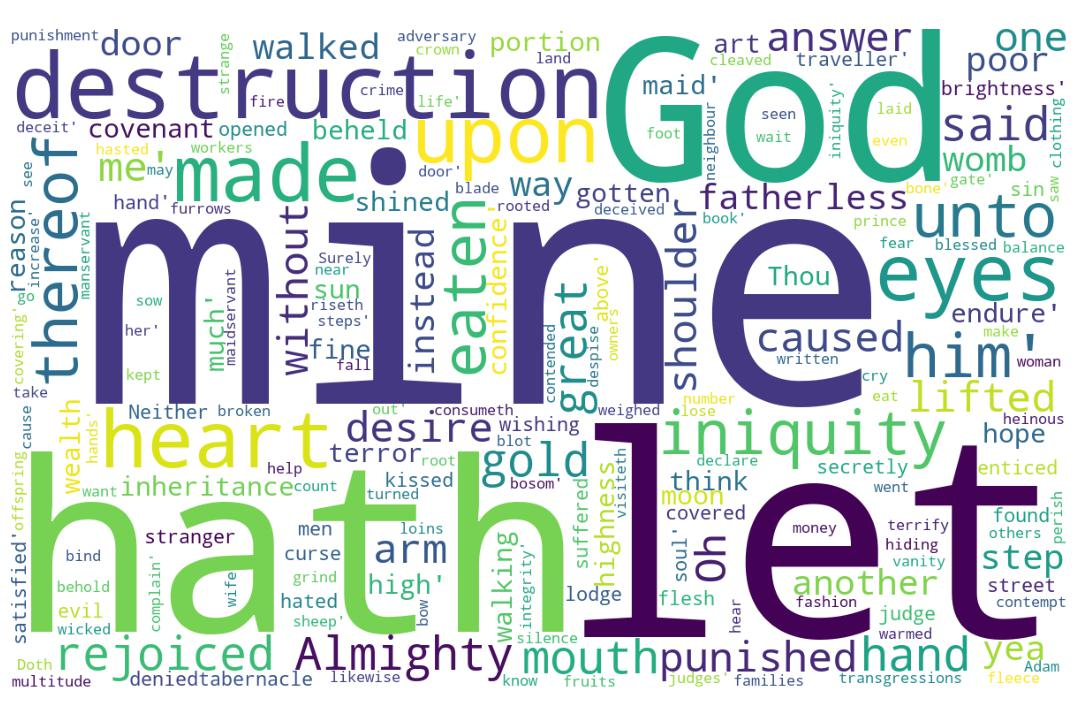
\includegraphics[width=\linewidth]{18OT-Job/Job31-WordCloud.jpg}
  \caption{Job 31 Word Cloud}
  \label{fig:Job 31 word Cloud}
\end{figure}


\marginpar{\scriptsize \centering \fcolorbox{bone}{lime}{\textbf{STILL MORE FROM JOB}}\\ (Job 31:1-40) \begin{compactenum}[I.][8]
    \item Job's \textbf{Decision(s)} to do Right \index[scripture]{Job!Job 31:01}(Job 31:1)
    \item Job has not been \textbf{Deceived}  \index[scripture]{Job!Job 31:09}(Job 31:9)
    \item Job knows \textbf{Destruction} is a Result of Sin (Judgment) \index[scripture]{Job!Job 31:12}(Job 31:12)
    \item Job has \textbf{Dealt} Mercifully with the Unfortunate \index[scripture]{Job!Job 31:21}(Job 31:21)
%    \item Job knows \textbf{Deliverance} is from God (Judgment) \index[scripture]{Job!Job 31:24}(Job 31:24)
    \item Job does not wish \textbf{Destruction} for his Enemies) \index[scripture]{Job!Job 31:29}(Job 31:29)
    \item Job \textbf{Desires} to Know his Account with God \index[scripture]{Job!Job 31:35}(Job 31:35)
    \item Job can \textbf{Declare} his Steps to God \index[scripture]{Job!Job 31:37}(Job 31:37)
\end{compactenum}}

\footnote{\textcolor[cmyk]{0.99998,1,0,0}{\hyperlink{TOC}{Return to end of Table of Contents.}}}\footnote{\href{https://www.audioverse.org/english/audiobibles/books/ENGKJV/O/Job/1}{\textcolor[cmyk]{0.99998,1,0,0}{Job  Audio}}}\textcolor[cmyk]{0.99998,1,0,0}{I made a \fcolorbox{bone}{lime}{covenant} with mine eyes; why then should I think upon a maid?}
[2] \textcolor[cmyk]{0.99998,1,0,0}{For what portion of God \emph{is} \emph{there} from above? and \emph{what} inheritance of the Almighty from on high?}
[3] \textcolor[cmyk]{0.99998,1,0,0}{\emph{Is} not destruction \fcolorbox{bone}{bone}{to}  the wicked? and a strange \emph{punishment} \fcolorbox{bone}{bone}{to}  the workers of iniquity?}
[4] \textcolor[cmyk]{0.99998,1,0,0}{Doth not he see my ways, and count all my steps?}
[5] \textcolor[cmyk]{0.99998,1,0,0}{If I have walked with vanity, or if my foot hath hasted \fcolorbox{bone}{bone}{to}  deceit;}
[6] \textcolor[cmyk]{0.99998,1,0,0}{Let \fcolorbox{bone}{bone}{me}  be weighed in an even balance, that God may know mine integrity.}
[7] \textcolor[cmyk]{0.99998,1,0,0}{If my step hath turned out of the way, and mine heart walked after mine eyes, and if any blot hath cleaved \fcolorbox{bone}{bone}{to}  mine hands;}
[8] \textcolor[cmyk]{0.99998,1,0,0}{\emph{Then} let \fcolorbox{bone}{bone}{me}  sow, and let another eat; yea, let my offspring be rooted out.}
[9] \textcolor[cmyk]{0.99998,1,0,0}{If mine heart have been \fcolorbox{bone}{lime}{deceived} by a woman, or \emph{if} I have laid wait at my neighbour's door;}
[10] \textcolor[cmyk]{0.99998,1,0,0}{\emph{Then} let my wife grind unto another, and let others bow down upon her.}
[11] \textcolor[cmyk]{0.99998,1,0,0}{For this \emph{is} an heinous crime; yea, it \emph{is} an iniquity \emph{to} \emph{be} \emph{punished} \emph{by} the judges.}
[12] \textcolor[cmyk]{0.99998,1,0,0}{For it \emph{is} a fire \emph{that} consumeth \fcolorbox{bone}{bone}{to}  \fcolorbox{bone}{lime}{destruction}, and would root out all mine increase.}
[13] \textcolor[cmyk]{0.99998,1,0,0}{If I did despise the cause of my manservant or of my maidservant, when they contended with \fcolorbox{bone}{bone}{me} ;}
[14] \textcolor[cmyk]{0.99998,1,0,0}{What then shall I do when God riseth up? and when he visiteth, what shall I answer him?}
[15] \textcolor[cmyk]{0.99998,1,0,0}{Did not he that made \fcolorbox{bone}{bone}{me}  in the womb make him? and did not one fashion us in the womb?}
[16] \textcolor[cmyk]{0.99998,1,0,0}{If I have withheld the poor from \emph{their} desire, or have caused the eyes of the widow \fcolorbox{bone}{bone}{to}  fail;}
[17] \textcolor[cmyk]{0.99998,1,0,0}{Or have eaten my morsel myself alone, and the fatherless hath not eaten thereof;}
[18] \textcolor[cmyk]{0.99998,1,0,0}{(For from my youth he was brought up with \fcolorbox{bone}{bone}{me} , as \emph{with} a father, and I have guided her from my mother's womb;)}
[19] \textcolor[cmyk]{0.99998,1,0,0}{If I have seen any perish for want of clothing, or any poor without covering;}
[20] \textcolor[cmyk]{0.99998,1,0,0}{If his loins have not blessed \fcolorbox{bone}{bone}{me} , and \emph{if} he were \emph{not} warmed with the fleece of my sheep;}
[21] \textcolor[cmyk]{0.99998,1,0,0}{If I have lifted up my hand \fcolorbox{bone}{lime}{against the fatherless}, when I saw my help in the gate:}
[22] \textcolor[cmyk]{0.99998,1,0,0}{\emph{Then} let mine arm fall from my shoulder blade, and mine arm be broken from the bone.}
[23] \textcolor[cmyk]{0.99998,1,0,0}{For destruction \emph{from} God \emph{was} a terror \fcolorbox{bone}{bone}{to}  \fcolorbox{bone}{bone}{me} , and by reason of his highness I could not endure.}
[24] \textcolor[cmyk]{0.99998,1,0,0}{If I have made gold my hope, or have said \fcolorbox{bone}{bone}{to}  the fine gold, \emph{Thou} \emph{art} my confidence;}
[25] \textcolor[cmyk]{0.99998,1,0,0}{If I rejoiced because my wealth \emph{was} great, and because mine hand had gotten much;}
[26] \textcolor[cmyk]{0.99998,1,0,0}{If I beheld the sun when it shined, or the moon walking \emph{in} brightness;}
[27] \textcolor[cmyk]{0.99998,1,0,0}{And my heart hath been secretly enticed, or my mouth hath kissed my hand:}
[28] \textcolor[cmyk]{0.99998,1,0,0}{This also \emph{were} an iniquity \emph{to} \emph{be} \emph{punished} \emph{by} the judge: for I should have denied the God \emph{that} \emph{is} above.}
[29] \textcolor[cmyk]{0.99998,1,0,0}{If I rejoiced at the destruction of him that hated \fcolorbox{bone}{bone}{me} , or lifted up myself when evil found him:}
[30] \textcolor[cmyk]{0.99998,1,0,0}{Neither have I suffered my mouth \fcolorbox{bone}{bone}{to}  sin by wishing a curse \fcolorbox{bone}{bone}{to}  his soul.}
[31] \textcolor[cmyk]{0.99998,1,0,0}{If the men of my tabernacle said not, Oh that we had of his flesh! we cannot be satisfied.}
[32] \textcolor[cmyk]{0.99998,1,0,0}{The stranger did not lodge in the street: \emph{but} I opened my doors \fcolorbox{bone}{bone}{to}  the traveller.}
[33] \textcolor[cmyk]{0.99998,1,0,0}{If I covered my transgressions as Adam, by hiding mine iniquity in my bosom:}
[34] \textcolor[cmyk]{0.99998,1,0,0}{Did I fear a great multitude, or did the contempt of families terrify \fcolorbox{bone}{bone}{me} , that I kept silence, \emph{and} went not out of the door?}
[35] \textcolor[cmyk]{0.99998,1,0,0}{Oh that one would hear \fcolorbox{bone}{bone}{me} ! behold, my \fcolorbox{bone}{lime}{desire} \emph{is,} \emph{that} the Almighty would answer \fcolorbox{bone}{bone}{me} , and \emph{that} mine adversary had written a book.}
[36] \textcolor[cmyk]{0.99998,1,0,0}{Surely I would take it upon my shoulder, \emph{and} bind it \emph{as} a crown \fcolorbox{bone}{bone}{to}  \fcolorbox{bone}{bone}{me} .}
[37] \textcolor[cmyk]{0.99998,1,0,0}{I would \fcolorbox{bone}{lime}{declare} unto him the number of my steps; as a prince would I go near unto him.}
[38] \textcolor[cmyk]{0.99998,1,0,0}{If my land cry against \fcolorbox{bone}{bone}{me} , or that the furrows likewise thereof complain;}
[39] \textcolor[cmyk]{0.99998,1,0,0}{If I have eaten the fruits thereof without money, or have caused the owners thereof \fcolorbox{bone}{bone}{to}  lose their life:}
[40] \textcolor[cmyk]{0.99998,1,0,0}{Let thistles grow instead of wheat, and cockle instead of barley. The words of Job are ended.}
\section{Job 31  Comments}

\subsection{Numeric Nuggets}
\textbf{13:} Verse 38 has 13 words. Verses 1, 3, 8, 10, 17, 26, 33, and 38 have 13 unique words. The words ``me'' and ``to'' are found 13 times in the chapter.

\subsection{Job 31 Introduction}
In chapter 31, Job presents his summary argument in defense, his resume of goodness.  It is an impressive list: \cite{ruckman1993Job}
\begin{compactenum}
    \item Job had no lust in his heart [1]
    \item Job kept faithful to his wife
    \item Job treated servants correctly
    \item Job considered the poor and the orphans
    \item Job didn't chase after riches [24]
    \item Job had no worldliness [24]
    \item Job carried out no vengeance [29]
    \item Job had no idolatry [26]
    \item Job did not rejoice over others' misfortune an djudgment [29,30]
    \item item Job had no cursing [30]
    \item Job had no deceit [34]
    \item Job had no stinginess [32]
    \item Job did not cover up sin [33]
    \item Job showed hospitality [34]
    \item Job had no compromising [35]
    \item Job had no stealing [39]
    \item Job had no wastefulness [40]
\end{compactenum}



\subsection{Job 31:1}
This is the anti-pornography verse.  Don't look because of what you will probably end up thinking.\cite{thomas_20220119}
\index[NWIV]{15!Job!Job 31:1}\index[AWIP]{I!Job!Job 31:1}\index[AWIP]{I!Job!Job 31:1 (2)}\index[AWIP]{made!Job!Job 31:1}\index[AWIP]{a!Job!Job 31:1}\index[AWIP]{a!Job!Job 31:1 (2)}\index[AWIP]{covenant!Job!Job 31:1}\index[AWIP]{with!Job!Job 31:1}\index[AWIP]{mine!Job!Job 31:1}\index[AWIP]{eyes!Job!Job 31:1}\index[AWIP]{why!Job!Job 31:1}\index[AWIP]{then!Job!Job 31:1}\index[AWIP]{should!Job!Job 31:1}\index[AWIP]{think!Job!Job 31:1}\index[AWIP]{upon!Job!Job 31:1}\index[AWIP]{maid?!Job!Job 31:1}

\index[NWIV]{18!Job!Job 31:2}\index[AWIP]{For!Job!Job 31:2}\index[AWIP]{what!Job!Job 31:2}\index[AWIP]{portion!Job!Job 31:2}\index[AWIP]{of!Job!Job 31:2}\index[AWIP]{of!Job!Job 31:2 (2)}\index[AWIP]{God!Job!Job 31:2}\index[AWIP]{\emph{is}!Job!Job 31:2}\index[AWIP]{\emph{there}!Job!Job 31:2}\index[AWIP]{from!Job!Job 31:2}\index[AWIP]{from!Job!Job 31:2 (2)}\index[AWIP]{above?!Job!Job 31:2}\index[AWIP]{and!Job!Job 31:2}\index[AWIP]{\emph{what}!Job!Job 31:2}\index[AWIP]{inheritance!Job!Job 31:2}\index[AWIP]{the!Job!Job 31:2}\index[AWIP]{Almighty!Job!Job 31:2}\index[AWIP]{on!Job!Job 31:2}\index[AWIP]{high?!Job!Job 31:2}\index[AWIP]{\emph{is}!Job!Job 31:2}\index[AWIP]{\emph{there}!Job!Job 31:2}\index[AWIP]{\emph{what}!Job!Job 31:2}

\index[NWIV]{15!Job!Job 31:3}\index[AWIP]{\emph{Is}!Job!Job 31:3}\index[AWIP]{not!Job!Job 31:3}\index[AWIP]{destruction!Job!Job 31:3}\index[AWIP]{to!Job!Job 31:3}\index[AWIP]{to!Job!Job 31:3 (2)}\index[AWIP]{the!Job!Job 31:3}\index[AWIP]{the!Job!Job 31:3 (2)}\index[AWIP]{wicked?!Job!Job 31:3}\index[AWIP]{and!Job!Job 31:3}\index[AWIP]{a!Job!Job 31:3}\index[AWIP]{strange!Job!Job 31:3}\index[AWIP]{\emph{punishment}!Job!Job 31:3}\index[AWIP]{workers!Job!Job 31:3}\index[AWIP]{of!Job!Job 31:3}\index[AWIP]{iniquity?!Job!Job 31:3}\index[AWIP]{\emph{Is}!Job!Job 31:3}\index[AWIP]{\emph{punishment}!Job!Job 31:3}

\index[NWIV]{11!Job!Job 31:4}\index[AWIP]{Doth!Job!Job 31:4}\index[AWIP]{not!Job!Job 31:4}\index[AWIP]{he!Job!Job 31:4}\index[AWIP]{see!Job!Job 31:4}\index[AWIP]{my!Job!Job 31:4}\index[AWIP]{my!Job!Job 31:4 (2)}\index[AWIP]{ways!Job!Job 31:4}\index[AWIP]{and!Job!Job 31:4}\index[AWIP]{count!Job!Job 31:4}\index[AWIP]{all!Job!Job 31:4}\index[AWIP]{steps?!Job!Job 31:4}

\index[NWIV]{14!Job!Job 31:5}\index[AWIP]{If!Job!Job 31:5}\index[AWIP]{I!Job!Job 31:5}\index[AWIP]{have!Job!Job 31:5}\index[AWIP]{walked!Job!Job 31:5}\index[AWIP]{with!Job!Job 31:5}\index[AWIP]{vanity!Job!Job 31:5}\index[AWIP]{or!Job!Job 31:5}\index[AWIP]{if!Job!Job 31:5}\index[AWIP]{my!Job!Job 31:5}\index[AWIP]{foot!Job!Job 31:5}\index[AWIP]{hath!Job!Job 31:5}\index[AWIP]{hasted!Job!Job 31:5}\index[AWIP]{to!Job!Job 31:5}\index[AWIP]{deceit!Job!Job 31:5}

\index[NWIV]{14!Job!Job 31:6}\index[AWIP]{Let!Job!Job 31:6}\index[AWIP]{me!Job!Job 31:6}\index[AWIP]{be!Job!Job 31:6}\index[AWIP]{weighed!Job!Job 31:6}\index[AWIP]{in!Job!Job 31:6}\index[AWIP]{an!Job!Job 31:6}\index[AWIP]{even!Job!Job 31:6}\index[AWIP]{balance!Job!Job 31:6}\index[AWIP]{that!Job!Job 31:6}\index[AWIP]{God!Job!Job 31:6}\index[AWIP]{may!Job!Job 31:6}\index[AWIP]{know!Job!Job 31:6}\index[AWIP]{mine!Job!Job 31:6}\index[AWIP]{integrity!Job!Job 31:6}

\index[NWIV]{25!Job!Job 31:7}\index[AWIP]{If!Job!Job 31:7}\index[AWIP]{my!Job!Job 31:7}\index[AWIP]{step!Job!Job 31:7}\index[AWIP]{hath!Job!Job 31:7}\index[AWIP]{hath!Job!Job 31:7 (2)}\index[AWIP]{turned!Job!Job 31:7}\index[AWIP]{out!Job!Job 31:7}\index[AWIP]{of!Job!Job 31:7}\index[AWIP]{the!Job!Job 31:7}\index[AWIP]{way!Job!Job 31:7}\index[AWIP]{and!Job!Job 31:7}\index[AWIP]{and!Job!Job 31:7 (2)}\index[AWIP]{mine!Job!Job 31:7}\index[AWIP]{mine!Job!Job 31:7 (2)}\index[AWIP]{mine!Job!Job 31:7 (3)}\index[AWIP]{heart!Job!Job 31:7}\index[AWIP]{walked!Job!Job 31:7}\index[AWIP]{after!Job!Job 31:7}\index[AWIP]{eyes!Job!Job 31:7}\index[AWIP]{if!Job!Job 31:7}\index[AWIP]{any!Job!Job 31:7}\index[AWIP]{blot!Job!Job 31:7}\index[AWIP]{cleaved!Job!Job 31:7}\index[AWIP]{to!Job!Job 31:7}\index[AWIP]{hands!Job!Job 31:7}

\index[NWIV]{15!Job!Job 31:8}\index[AWIP]{\emph{Then}!Job!Job 31:8}\index[AWIP]{let!Job!Job 31:8}\index[AWIP]{let!Job!Job 31:8 (2)}\index[AWIP]{let!Job!Job 31:8 (3)}\index[AWIP]{me!Job!Job 31:8}\index[AWIP]{sow!Job!Job 31:8}\index[AWIP]{and!Job!Job 31:8}\index[AWIP]{another!Job!Job 31:8}\index[AWIP]{eat!Job!Job 31:8}\index[AWIP]{yea!Job!Job 31:8}\index[AWIP]{my!Job!Job 31:8}\index[AWIP]{offspring!Job!Job 31:8}\index[AWIP]{be!Job!Job 31:8}\index[AWIP]{rooted!Job!Job 31:8}\index[AWIP]{out!Job!Job 31:8}\index[AWIP]{\emph{Then}!Job!Job 31:8}

\index[NWIV]{19!Job!Job 31:9}\index[AWIP]{If!Job!Job 31:9}\index[AWIP]{mine!Job!Job 31:9}\index[AWIP]{heart!Job!Job 31:9}\index[AWIP]{have!Job!Job 31:9}\index[AWIP]{have!Job!Job 31:9 (2)}\index[AWIP]{been!Job!Job 31:9}\index[AWIP]{deceived!Job!Job 31:9}\index[AWIP]{by!Job!Job 31:9}\index[AWIP]{a!Job!Job 31:9}\index[AWIP]{woman!Job!Job 31:9}\index[AWIP]{or!Job!Job 31:9}\index[AWIP]{\emph{if}!Job!Job 31:9}\index[AWIP]{I!Job!Job 31:9}\index[AWIP]{laid!Job!Job 31:9}\index[AWIP]{wait!Job!Job 31:9}\index[AWIP]{at!Job!Job 31:9}\index[AWIP]{my!Job!Job 31:9}\index[AWIP]{neighbour's!Job!Job 31:9}\index[AWIP]{door!Job!Job 31:9}\index[AWIP]{\emph{if}!Job!Job 31:9}

\index[NWIV]{14!Job!Job 31:10}\index[AWIP]{\emph{Then}!Job!Job 31:10}\index[AWIP]{let!Job!Job 31:10}\index[AWIP]{let!Job!Job 31:10 (2)}\index[AWIP]{my!Job!Job 31:10}\index[AWIP]{wife!Job!Job 31:10}\index[AWIP]{grind!Job!Job 31:10}\index[AWIP]{unto!Job!Job 31:10}\index[AWIP]{another!Job!Job 31:10}\index[AWIP]{and!Job!Job 31:10}\index[AWIP]{others!Job!Job 31:10}\index[AWIP]{bow!Job!Job 31:10}\index[AWIP]{down!Job!Job 31:10}\index[AWIP]{upon!Job!Job 31:10}\index[AWIP]{her!Job!Job 31:10}\index[AWIP]{\emph{Then}!Job!Job 31:10}

\index[NWIV]{17!Job!Job 31:11}\index[AWIP]{For!Job!Job 31:11}\index[AWIP]{this!Job!Job 31:11}\index[AWIP]{\emph{is}!Job!Job 31:11}\index[AWIP]{\emph{is}!Job!Job 31:11 (2)}\index[AWIP]{an!Job!Job 31:11}\index[AWIP]{an!Job!Job 31:11 (2)}\index[AWIP]{heinous!Job!Job 31:11}\index[AWIP]{crime!Job!Job 31:11}\index[AWIP]{yea!Job!Job 31:11}\index[AWIP]{it!Job!Job 31:11}\index[AWIP]{iniquity!Job!Job 31:11}\index[AWIP]{\emph{to}!Job!Job 31:11}\index[AWIP]{\emph{be}!Job!Job 31:11}\index[AWIP]{\emph{punished}!Job!Job 31:11}\index[AWIP]{\emph{by}!Job!Job 31:11}\index[AWIP]{the!Job!Job 31:11}\index[AWIP]{judges!Job!Job 31:11}\index[AWIP]{\emph{is}!Job!Job 31:11}\index[AWIP]{\emph{is}!Job!Job 31:11 (2)}\index[AWIP]{\emph{to}!Job!Job 31:11}\index[AWIP]{\emph{be}!Job!Job 31:11}\index[AWIP]{\emph{punished}!Job!Job 31:11}\index[AWIP]{\emph{by}!Job!Job 31:11}

\index[NWIV]{16!Job!Job 31:12}\index[AWIP]{For!Job!Job 31:12}\index[AWIP]{it!Job!Job 31:12}\index[AWIP]{\emph{is}!Job!Job 31:12}\index[AWIP]{a!Job!Job 31:12}\index[AWIP]{fire!Job!Job 31:12}\index[AWIP]{\emph{that}!Job!Job 31:12}\index[AWIP]{consumeth!Job!Job 31:12}\index[AWIP]{to!Job!Job 31:12}\index[AWIP]{destruction!Job!Job 31:12}\index[AWIP]{and!Job!Job 31:12}\index[AWIP]{would!Job!Job 31:12}\index[AWIP]{root!Job!Job 31:12}\index[AWIP]{out!Job!Job 31:12}\index[AWIP]{all!Job!Job 31:12}\index[AWIP]{mine!Job!Job 31:12}\index[AWIP]{increase!Job!Job 31:12}\index[AWIP]{\emph{is}!Job!Job 31:12}\index[AWIP]{\emph{that}!Job!Job 31:12}

\index[NWIV]{18!Job!Job 31:13}\index[AWIP]{If!Job!Job 31:13}\index[AWIP]{I!Job!Job 31:13}\index[AWIP]{did!Job!Job 31:13}\index[AWIP]{despise!Job!Job 31:13}\index[AWIP]{the!Job!Job 31:13}\index[AWIP]{cause!Job!Job 31:13}\index[AWIP]{of!Job!Job 31:13}\index[AWIP]{of!Job!Job 31:13 (2)}\index[AWIP]{my!Job!Job 31:13}\index[AWIP]{my!Job!Job 31:13 (2)}\index[AWIP]{manservant!Job!Job 31:13}\index[AWIP]{or!Job!Job 31:13}\index[AWIP]{maidservant!Job!Job 31:13}\index[AWIP]{when!Job!Job 31:13}\index[AWIP]{they!Job!Job 31:13}\index[AWIP]{contended!Job!Job 31:13}\index[AWIP]{with!Job!Job 31:13}\index[AWIP]{me!Job!Job 31:13}

\index[NWIV]{18!Job!Job 31:14}\index[AWIP]{What!Job!Job 31:14}\index[AWIP]{then!Job!Job 31:14}\index[AWIP]{shall!Job!Job 31:14}\index[AWIP]{shall!Job!Job 31:14 (2)}\index[AWIP]{I!Job!Job 31:14}\index[AWIP]{I!Job!Job 31:14 (2)}\index[AWIP]{do!Job!Job 31:14}\index[AWIP]{when!Job!Job 31:14}\index[AWIP]{when!Job!Job 31:14 (2)}\index[AWIP]{God!Job!Job 31:14}\index[AWIP]{riseth!Job!Job 31:14}\index[AWIP]{up?!Job!Job 31:14}\index[AWIP]{and!Job!Job 31:14}\index[AWIP]{he!Job!Job 31:14}\index[AWIP]{visiteth!Job!Job 31:14}\index[AWIP]{what!Job!Job 31:14}\index[AWIP]{answer!Job!Job 31:14}\index[AWIP]{him?!Job!Job 31:14}

\index[NWIV]{20!Job!Job 31:15}\index[AWIP]{Did!Job!Job 31:15}\index[AWIP]{not!Job!Job 31:15}\index[AWIP]{not!Job!Job 31:15 (2)}\index[AWIP]{he!Job!Job 31:15}\index[AWIP]{that!Job!Job 31:15}\index[AWIP]{made!Job!Job 31:15}\index[AWIP]{me!Job!Job 31:15}\index[AWIP]{in!Job!Job 31:15}\index[AWIP]{in!Job!Job 31:15 (2)}\index[AWIP]{the!Job!Job 31:15}\index[AWIP]{the!Job!Job 31:15 (2)}\index[AWIP]{womb!Job!Job 31:15}\index[AWIP]{make!Job!Job 31:15}\index[AWIP]{him?!Job!Job 31:15}\index[AWIP]{and!Job!Job 31:15}\index[AWIP]{did!Job!Job 31:15}\index[AWIP]{one!Job!Job 31:15}\index[AWIP]{fashion!Job!Job 31:15}\index[AWIP]{us!Job!Job 31:15}\index[AWIP]{womb?!Job!Job 31:15}

\index[NWIV]{19!Job!Job 31:16}\index[AWIP]{If!Job!Job 31:16}\index[AWIP]{I!Job!Job 31:16}\index[AWIP]{have!Job!Job 31:16}\index[AWIP]{have!Job!Job 31:16 (2)}\index[AWIP]{withheld!Job!Job 31:16}\index[AWIP]{the!Job!Job 31:16}\index[AWIP]{the!Job!Job 31:16 (2)}\index[AWIP]{the!Job!Job 31:16 (3)}\index[AWIP]{poor!Job!Job 31:16}\index[AWIP]{from!Job!Job 31:16}\index[AWIP]{\emph{their}!Job!Job 31:16}\index[AWIP]{desire!Job!Job 31:16}\index[AWIP]{or!Job!Job 31:16}\index[AWIP]{caused!Job!Job 31:16}\index[AWIP]{eyes!Job!Job 31:16}\index[AWIP]{of!Job!Job 31:16}\index[AWIP]{widow!Job!Job 31:16}\index[AWIP]{to!Job!Job 31:16}\index[AWIP]{fail!Job!Job 31:16}\index[AWIP]{\emph{their}!Job!Job 31:16}

\index[NWIV]{14!Job!Job 31:17}\index[AWIP]{Or!Job!Job 31:17}\index[AWIP]{have!Job!Job 31:17}\index[AWIP]{eaten!Job!Job 31:17}\index[AWIP]{eaten!Job!Job 31:17 (2)}\index[AWIP]{my!Job!Job 31:17}\index[AWIP]{morsel!Job!Job 31:17}\index[AWIP]{myself!Job!Job 31:17}\index[AWIP]{alone!Job!Job 31:17}\index[AWIP]{and!Job!Job 31:17}\index[AWIP]{the!Job!Job 31:17}\index[AWIP]{fatherless!Job!Job 31:17}\index[AWIP]{hath!Job!Job 31:17}\index[AWIP]{not!Job!Job 31:17}\index[AWIP]{thereof!Job!Job 31:17}

\index[NWIV]{23!Job!Job 31:18}\index[AWIP]{(For!Job!Job 31:18}\index[AWIP]{from!Job!Job 31:18}\index[AWIP]{from!Job!Job 31:18 (2)}\index[AWIP]{my!Job!Job 31:18}\index[AWIP]{my!Job!Job 31:18 (2)}\index[AWIP]{youth!Job!Job 31:18}\index[AWIP]{he!Job!Job 31:18}\index[AWIP]{was!Job!Job 31:18}\index[AWIP]{brought!Job!Job 31:18}\index[AWIP]{up!Job!Job 31:18}\index[AWIP]{with!Job!Job 31:18}\index[AWIP]{me!Job!Job 31:18}\index[AWIP]{as!Job!Job 31:18}\index[AWIP]{\emph{with}!Job!Job 31:18}\index[AWIP]{a!Job!Job 31:18}\index[AWIP]{father!Job!Job 31:18}\index[AWIP]{and!Job!Job 31:18}\index[AWIP]{I!Job!Job 31:18}\index[AWIP]{have!Job!Job 31:18}\index[AWIP]{guided!Job!Job 31:18}\index[AWIP]{her!Job!Job 31:18}\index[AWIP]{mother's!Job!Job 31:18}\index[AWIP]{womb)!Job!Job 31:18}\index[AWIP]{\emph{with}!Job!Job 31:18}

\index[NWIV]{15!Job!Job 31:19}\index[AWIP]{If!Job!Job 31:19}\index[AWIP]{I!Job!Job 31:19}\index[AWIP]{have!Job!Job 31:19}\index[AWIP]{seen!Job!Job 31:19}\index[AWIP]{any!Job!Job 31:19}\index[AWIP]{any!Job!Job 31:19 (2)}\index[AWIP]{perish!Job!Job 31:19}\index[AWIP]{for!Job!Job 31:19}\index[AWIP]{want!Job!Job 31:19}\index[AWIP]{of!Job!Job 31:19}\index[AWIP]{clothing!Job!Job 31:19}\index[AWIP]{or!Job!Job 31:19}\index[AWIP]{poor!Job!Job 31:19}\index[AWIP]{without!Job!Job 31:19}\index[AWIP]{covering!Job!Job 31:19}

\index[NWIV]{19!Job!Job 31:20}\index[AWIP]{If!Job!Job 31:20}\index[AWIP]{his!Job!Job 31:20}\index[AWIP]{loins!Job!Job 31:20}\index[AWIP]{have!Job!Job 31:20}\index[AWIP]{not!Job!Job 31:20}\index[AWIP]{blessed!Job!Job 31:20}\index[AWIP]{me!Job!Job 31:20}\index[AWIP]{and!Job!Job 31:20}\index[AWIP]{\emph{if}!Job!Job 31:20}\index[AWIP]{he!Job!Job 31:20}\index[AWIP]{were!Job!Job 31:20}\index[AWIP]{\emph{not}!Job!Job 31:20}\index[AWIP]{warmed!Job!Job 31:20}\index[AWIP]{with!Job!Job 31:20}\index[AWIP]{the!Job!Job 31:20}\index[AWIP]{fleece!Job!Job 31:20}\index[AWIP]{of!Job!Job 31:20}\index[AWIP]{my!Job!Job 31:20}\index[AWIP]{sheep!Job!Job 31:20}\index[AWIP]{\emph{if}!Job!Job 31:20}\index[AWIP]{\emph{not}!Job!Job 31:20}

\index[NWIV]{18!Job!Job 31:21}\index[AWIP]{If!Job!Job 31:21}\index[AWIP]{I!Job!Job 31:21}\index[AWIP]{I!Job!Job 31:21 (2)}\index[AWIP]{have!Job!Job 31:21}\index[AWIP]{lifted!Job!Job 31:21}\index[AWIP]{up!Job!Job 31:21}\index[AWIP]{my!Job!Job 31:21}\index[AWIP]{my!Job!Job 31:21 (2)}\index[AWIP]{hand!Job!Job 31:21}\index[AWIP]{against!Job!Job 31:21}\index[AWIP]{the!Job!Job 31:21}\index[AWIP]{the!Job!Job 31:21 (2)}\index[AWIP]{fatherless!Job!Job 31:21}\index[AWIP]{when!Job!Job 31:21}\index[AWIP]{saw!Job!Job 31:21}\index[AWIP]{help!Job!Job 31:21}\index[AWIP]{in!Job!Job 31:21}\index[AWIP]{gate!Job!Job 31:21}

\index[NWIV]{17!Job!Job 31:22}\index[AWIP]{\emph{Then}!Job!Job 31:22}\index[AWIP]{let!Job!Job 31:22}\index[AWIP]{mine!Job!Job 31:22}\index[AWIP]{mine!Job!Job 31:22 (2)}\index[AWIP]{arm!Job!Job 31:22}\index[AWIP]{arm!Job!Job 31:22 (2)}\index[AWIP]{fall!Job!Job 31:22}\index[AWIP]{from!Job!Job 31:22}\index[AWIP]{from!Job!Job 31:22 (2)}\index[AWIP]{my!Job!Job 31:22}\index[AWIP]{shoulder!Job!Job 31:22}\index[AWIP]{blade!Job!Job 31:22}\index[AWIP]{and!Job!Job 31:22}\index[AWIP]{be!Job!Job 31:22}\index[AWIP]{broken!Job!Job 31:22}\index[AWIP]{the!Job!Job 31:22}\index[AWIP]{bone!Job!Job 31:22}\index[AWIP]{\emph{Then}!Job!Job 31:22}

\index[NWIV]{19!Job!Job 31:23}\index[AWIP]{For!Job!Job 31:23}\index[AWIP]{destruction!Job!Job 31:23}\index[AWIP]{\emph{from}!Job!Job 31:23}\index[AWIP]{God!Job!Job 31:23}\index[AWIP]{\emph{was}!Job!Job 31:23}\index[AWIP]{a!Job!Job 31:23}\index[AWIP]{terror!Job!Job 31:23}\index[AWIP]{to!Job!Job 31:23}\index[AWIP]{me!Job!Job 31:23}\index[AWIP]{and!Job!Job 31:23}\index[AWIP]{by!Job!Job 31:23}\index[AWIP]{reason!Job!Job 31:23}\index[AWIP]{of!Job!Job 31:23}\index[AWIP]{his!Job!Job 31:23}\index[AWIP]{highness!Job!Job 31:23}\index[AWIP]{I!Job!Job 31:23}\index[AWIP]{could!Job!Job 31:23}\index[AWIP]{not!Job!Job 31:23}\index[AWIP]{endure!Job!Job 31:23}\index[AWIP]{\emph{from}!Job!Job 31:23}\index[AWIP]{\emph{was}!Job!Job 31:23}

\index[NWIV]{18!Job!Job 31:24}\index[AWIP]{If!Job!Job 31:24}\index[AWIP]{I!Job!Job 31:24}\index[AWIP]{have!Job!Job 31:24}\index[AWIP]{have!Job!Job 31:24 (2)}\index[AWIP]{made!Job!Job 31:24}\index[AWIP]{gold!Job!Job 31:24}\index[AWIP]{gold!Job!Job 31:24 (2)}\index[AWIP]{my!Job!Job 31:24}\index[AWIP]{my!Job!Job 31:24 (2)}\index[AWIP]{hope!Job!Job 31:24}\index[AWIP]{or!Job!Job 31:24}\index[AWIP]{said!Job!Job 31:24}\index[AWIP]{to!Job!Job 31:24}\index[AWIP]{the!Job!Job 31:24}\index[AWIP]{fine!Job!Job 31:24}\index[AWIP]{\emph{Thou}!Job!Job 31:24}\index[AWIP]{\emph{art}!Job!Job 31:24}\index[AWIP]{confidence!Job!Job 31:24}\index[AWIP]{\emph{Thou}!Job!Job 31:24}\index[AWIP]{\emph{art}!Job!Job 31:24}

\index[NWIV]{15!Job!Job 31:25}\index[AWIP]{If!Job!Job 31:25}\index[AWIP]{I!Job!Job 31:25}\index[AWIP]{rejoiced!Job!Job 31:25}\index[AWIP]{because!Job!Job 31:25}\index[AWIP]{because!Job!Job 31:25 (2)}\index[AWIP]{my!Job!Job 31:25}\index[AWIP]{wealth!Job!Job 31:25}\index[AWIP]{\emph{was}!Job!Job 31:25}\index[AWIP]{great!Job!Job 31:25}\index[AWIP]{and!Job!Job 31:25}\index[AWIP]{mine!Job!Job 31:25}\index[AWIP]{hand!Job!Job 31:25}\index[AWIP]{had!Job!Job 31:25}\index[AWIP]{gotten!Job!Job 31:25}\index[AWIP]{much!Job!Job 31:25}\index[AWIP]{\emph{was}!Job!Job 31:25}

\index[NWIV]{14!Job!Job 31:26}\index[AWIP]{If!Job!Job 31:26}\index[AWIP]{I!Job!Job 31:26}\index[AWIP]{beheld!Job!Job 31:26}\index[AWIP]{the!Job!Job 31:26}\index[AWIP]{the!Job!Job 31:26 (2)}\index[AWIP]{sun!Job!Job 31:26}\index[AWIP]{when!Job!Job 31:26}\index[AWIP]{it!Job!Job 31:26}\index[AWIP]{shined!Job!Job 31:26}\index[AWIP]{or!Job!Job 31:26}\index[AWIP]{moon!Job!Job 31:26}\index[AWIP]{walking!Job!Job 31:26}\index[AWIP]{\emph{in}!Job!Job 31:26}\index[AWIP]{brightness!Job!Job 31:26}\index[AWIP]{\emph{in}!Job!Job 31:26}

\index[NWIV]{14!Job!Job 31:27}\index[AWIP]{And!Job!Job 31:27}\index[AWIP]{my!Job!Job 31:27}\index[AWIP]{my!Job!Job 31:27 (2)}\index[AWIP]{my!Job!Job 31:27 (3)}\index[AWIP]{heart!Job!Job 31:27}\index[AWIP]{hath!Job!Job 31:27}\index[AWIP]{hath!Job!Job 31:27 (2)}\index[AWIP]{been!Job!Job 31:27}\index[AWIP]{secretly!Job!Job 31:27}\index[AWIP]{enticed!Job!Job 31:27}\index[AWIP]{or!Job!Job 31:27}\index[AWIP]{mouth!Job!Job 31:27}\index[AWIP]{kissed!Job!Job 31:27}\index[AWIP]{hand!Job!Job 31:27}

\index[NWIV]{21!Job!Job 31:28}\index[AWIP]{This!Job!Job 31:28}\index[AWIP]{also!Job!Job 31:28}\index[AWIP]{\emph{were}!Job!Job 31:28}\index[AWIP]{an!Job!Job 31:28}\index[AWIP]{iniquity!Job!Job 31:28}\index[AWIP]{\emph{to}!Job!Job 31:28}\index[AWIP]{\emph{be}!Job!Job 31:28}\index[AWIP]{\emph{punished}!Job!Job 31:28}\index[AWIP]{\emph{by}!Job!Job 31:28}\index[AWIP]{the!Job!Job 31:28}\index[AWIP]{the!Job!Job 31:28 (2)}\index[AWIP]{judge!Job!Job 31:28}\index[AWIP]{for!Job!Job 31:28}\index[AWIP]{I!Job!Job 31:28}\index[AWIP]{should!Job!Job 31:28}\index[AWIP]{have!Job!Job 31:28}\index[AWIP]{denied!Job!Job 31:28}\index[AWIP]{God!Job!Job 31:28}\index[AWIP]{\emph{that}!Job!Job 31:28}\index[AWIP]{\emph{is}!Job!Job 31:28}\index[AWIP]{above!Job!Job 31:28}\index[AWIP]{\emph{were}!Job!Job 31:28}\index[AWIP]{\emph{to}!Job!Job 31:28}\index[AWIP]{\emph{be}!Job!Job 31:28}\index[AWIP]{\emph{punished}!Job!Job 31:28}\index[AWIP]{\emph{by}!Job!Job 31:28}\index[AWIP]{\emph{that}!Job!Job 31:28}\index[AWIP]{\emph{is}!Job!Job 31:28}

\index[NWIV]{19!Job!Job 31:29}\index[AWIP]{If!Job!Job 31:29}\index[AWIP]{I!Job!Job 31:29}\index[AWIP]{rejoiced!Job!Job 31:29}\index[AWIP]{at!Job!Job 31:29}\index[AWIP]{the!Job!Job 31:29}\index[AWIP]{destruction!Job!Job 31:29}\index[AWIP]{of!Job!Job 31:29}\index[AWIP]{him!Job!Job 31:29}\index[AWIP]{him!Job!Job 31:29 (2)}\index[AWIP]{that!Job!Job 31:29}\index[AWIP]{hated!Job!Job 31:29}\index[AWIP]{me!Job!Job 31:29}\index[AWIP]{or!Job!Job 31:29}\index[AWIP]{lifted!Job!Job 31:29}\index[AWIP]{up!Job!Job 31:29}\index[AWIP]{myself!Job!Job 31:29}\index[AWIP]{when!Job!Job 31:29}\index[AWIP]{evil!Job!Job 31:29}\index[AWIP]{found!Job!Job 31:29}

\index[NWIV]{15!Job!Job 31:30}\index[AWIP]{Neither!Job!Job 31:30}\index[AWIP]{have!Job!Job 31:30}\index[AWIP]{I!Job!Job 31:30}\index[AWIP]{suffered!Job!Job 31:30}\index[AWIP]{my!Job!Job 31:30}\index[AWIP]{mouth!Job!Job 31:30}\index[AWIP]{to!Job!Job 31:30}\index[AWIP]{to!Job!Job 31:30 (2)}\index[AWIP]{sin!Job!Job 31:30}\index[AWIP]{by!Job!Job 31:30}\index[AWIP]{wishing!Job!Job 31:30}\index[AWIP]{a!Job!Job 31:30}\index[AWIP]{curse!Job!Job 31:30}\index[AWIP]{his!Job!Job 31:30}\index[AWIP]{soul!Job!Job 31:30}

\index[NWIV]{19!Job!Job 31:31}\index[AWIP]{If!Job!Job 31:31}\index[AWIP]{the!Job!Job 31:31}\index[AWIP]{men!Job!Job 31:31}\index[AWIP]{of!Job!Job 31:31}\index[AWIP]{of!Job!Job 31:31 (2)}\index[AWIP]{my!Job!Job 31:31}\index[AWIP]{tabernacle!Job!Job 31:31}\index[AWIP]{said!Job!Job 31:31}\index[AWIP]{not!Job!Job 31:31}\index[AWIP]{Oh!Job!Job 31:31}\index[AWIP]{that!Job!Job 31:31}\index[AWIP]{we!Job!Job 31:31}\index[AWIP]{we!Job!Job 31:31 (2)}\index[AWIP]{had!Job!Job 31:31}\index[AWIP]{his!Job!Job 31:31}\index[AWIP]{flesh!!Job!Job 31:31}\index[AWIP]{cannot!Job!Job 31:31}\index[AWIP]{be!Job!Job 31:31}\index[AWIP]{satisfied!Job!Job 31:31}

\index[NWIV]{16!Job!Job 31:32}\index[AWIP]{The!Job!Job 31:32}\index[AWIP]{stranger!Job!Job 31:32}\index[AWIP]{did!Job!Job 31:32}\index[AWIP]{not!Job!Job 31:32}\index[AWIP]{lodge!Job!Job 31:32}\index[AWIP]{in!Job!Job 31:32}\index[AWIP]{the!Job!Job 31:32}\index[AWIP]{the!Job!Job 31:32 (2)}\index[AWIP]{street!Job!Job 31:32}\index[AWIP]{\emph{but}!Job!Job 31:32}\index[AWIP]{I!Job!Job 31:32}\index[AWIP]{opened!Job!Job 31:32}\index[AWIP]{my!Job!Job 31:32}\index[AWIP]{doors!Job!Job 31:32}\index[AWIP]{to!Job!Job 31:32}\index[AWIP]{traveller!Job!Job 31:32}\index[AWIP]{\emph{but}!Job!Job 31:32}

\index[NWIV]{14!Job!Job 31:33}\index[AWIP]{If!Job!Job 31:33}\index[AWIP]{I!Job!Job 31:33}\index[AWIP]{covered!Job!Job 31:33}\index[AWIP]{my!Job!Job 31:33}\index[AWIP]{my!Job!Job 31:33 (2)}\index[AWIP]{transgressions!Job!Job 31:33}\index[AWIP]{as!Job!Job 31:33}\index[AWIP]{Adam!Job!Job 31:33}\index[AWIP]{by!Job!Job 31:33}\index[AWIP]{hiding!Job!Job 31:33}\index[AWIP]{mine!Job!Job 31:33}\index[AWIP]{iniquity!Job!Job 31:33}\index[AWIP]{in!Job!Job 31:33}\index[AWIP]{bosom!Job!Job 31:33}

\index[NWIV]{25!Job!Job 31:34}\index[AWIP]{Did!Job!Job 31:34}\index[AWIP]{I!Job!Job 31:34}\index[AWIP]{I!Job!Job 31:34 (2)}\index[AWIP]{fear!Job!Job 31:34}\index[AWIP]{a!Job!Job 31:34}\index[AWIP]{great!Job!Job 31:34}\index[AWIP]{multitude!Job!Job 31:34}\index[AWIP]{or!Job!Job 31:34}\index[AWIP]{did!Job!Job 31:34}\index[AWIP]{the!Job!Job 31:34}\index[AWIP]{the!Job!Job 31:34 (2)}\index[AWIP]{contempt!Job!Job 31:34}\index[AWIP]{of!Job!Job 31:34}\index[AWIP]{of!Job!Job 31:34 (2)}\index[AWIP]{families!Job!Job 31:34}\index[AWIP]{terrify!Job!Job 31:34}\index[AWIP]{me!Job!Job 31:34}\index[AWIP]{that!Job!Job 31:34}\index[AWIP]{kept!Job!Job 31:34}\index[AWIP]{silence!Job!Job 31:34}\index[AWIP]{\emph{and}!Job!Job 31:34}\index[AWIP]{went!Job!Job 31:34}\index[AWIP]{not!Job!Job 31:34}\index[AWIP]{out!Job!Job 31:34}\index[AWIP]{door?!Job!Job 31:34}\index[AWIP]{\emph{and}!Job!Job 31:34}

\index[NWIV]{24!Job!Job 31:35}\index[AWIP]{Oh!Job!Job 31:35}\index[AWIP]{that!Job!Job 31:35}\index[AWIP]{one!Job!Job 31:35}\index[AWIP]{would!Job!Job 31:35}\index[AWIP]{would!Job!Job 31:35 (2)}\index[AWIP]{hear!Job!Job 31:35}\index[AWIP]{me!!Job!Job 31:35}\index[AWIP]{behold!Job!Job 31:35}\index[AWIP]{my!Job!Job 31:35}\index[AWIP]{desire!Job!Job 31:35}\index[AWIP]{\emph{is}!Job!Job 31:35}\index[AWIP]{\emph{that}!Job!Job 31:35}\index[AWIP]{\emph{that}!Job!Job 31:35 (2)}\index[AWIP]{the!Job!Job 31:35}\index[AWIP]{Almighty!Job!Job 31:35}\index[AWIP]{answer!Job!Job 31:35}\index[AWIP]{me!Job!Job 31:35}\index[AWIP]{and!Job!Job 31:35}\index[AWIP]{mine!Job!Job 31:35}\index[AWIP]{adversary!Job!Job 31:35}\index[AWIP]{had!Job!Job 31:35}\index[AWIP]{written!Job!Job 31:35}\index[AWIP]{a!Job!Job 31:35}\index[AWIP]{book!Job!Job 31:35}\index[AWIP]{\emph{is}!Job!Job 31:35}\index[AWIP]{\emph{that}!Job!Job 31:35}\index[AWIP]{\emph{that}!Job!Job 31:35 (2)}

\index[NWIV]{16!Job!Job 31:36}\index[AWIP]{Surely!Job!Job 31:36}\index[AWIP]{I!Job!Job 31:36}\index[AWIP]{would!Job!Job 31:36}\index[AWIP]{take!Job!Job 31:36}\index[AWIP]{it!Job!Job 31:36}\index[AWIP]{it!Job!Job 31:36 (2)}\index[AWIP]{upon!Job!Job 31:36}\index[AWIP]{my!Job!Job 31:36}\index[AWIP]{shoulder!Job!Job 31:36}\index[AWIP]{\emph{and}!Job!Job 31:36}\index[AWIP]{bind!Job!Job 31:36}\index[AWIP]{\emph{as}!Job!Job 31:36}\index[AWIP]{a!Job!Job 31:36}\index[AWIP]{crown!Job!Job 31:36}\index[AWIP]{to!Job!Job 31:36}\index[AWIP]{me!Job!Job 31:36}\index[AWIP]{\emph{and}!Job!Job 31:36}\index[AWIP]{\emph{as}!Job!Job 31:36}

\index[NWIV]{19!Job!Job 31:37}\index[AWIP]{I!Job!Job 31:37}\index[AWIP]{I!Job!Job 31:37 (2)}\index[AWIP]{would!Job!Job 31:37}\index[AWIP]{would!Job!Job 31:37 (2)}\index[AWIP]{declare!Job!Job 31:37}\index[AWIP]{unto!Job!Job 31:37}\index[AWIP]{unto!Job!Job 31:37 (2)}\index[AWIP]{him!Job!Job 31:37}\index[AWIP]{him!Job!Job 31:37 (2)}\index[AWIP]{the!Job!Job 31:37}\index[AWIP]{number!Job!Job 31:37}\index[AWIP]{of!Job!Job 31:37}\index[AWIP]{my!Job!Job 31:37}\index[AWIP]{steps!Job!Job 31:37}\index[AWIP]{as!Job!Job 31:37}\index[AWIP]{a!Job!Job 31:37}\index[AWIP]{prince!Job!Job 31:37}\index[AWIP]{go!Job!Job 31:37}\index[AWIP]{near!Job!Job 31:37}

\index[NWIV]{13!Job!Job 31:38}\index[AWIP]{If!Job!Job 31:38}\index[AWIP]{my!Job!Job 31:38}\index[AWIP]{land!Job!Job 31:38}\index[AWIP]{cry!Job!Job 31:38}\index[AWIP]{against!Job!Job 31:38}\index[AWIP]{me!Job!Job 31:38}\index[AWIP]{or!Job!Job 31:38}\index[AWIP]{that!Job!Job 31:38}\index[AWIP]{the!Job!Job 31:38}\index[AWIP]{furrows!Job!Job 31:38}\index[AWIP]{likewise!Job!Job 31:38}\index[AWIP]{thereof!Job!Job 31:38}\index[AWIP]{complain!Job!Job 31:38}

\index[NWIV]{19!Job!Job 31:39}\index[AWIP]{If!Job!Job 31:39}\index[AWIP]{I!Job!Job 31:39}\index[AWIP]{have!Job!Job 31:39}\index[AWIP]{have!Job!Job 31:39 (2)}\index[AWIP]{eaten!Job!Job 31:39}\index[AWIP]{the!Job!Job 31:39}\index[AWIP]{the!Job!Job 31:39 (2)}\index[AWIP]{fruits!Job!Job 31:39}\index[AWIP]{thereof!Job!Job 31:39}\index[AWIP]{thereof!Job!Job 31:39 (2)}\index[AWIP]{without!Job!Job 31:39}\index[AWIP]{money!Job!Job 31:39}\index[AWIP]{or!Job!Job 31:39}\index[AWIP]{caused!Job!Job 31:39}\index[AWIP]{owners!Job!Job 31:39}\index[AWIP]{to!Job!Job 31:39}\index[AWIP]{lose!Job!Job 31:39}\index[AWIP]{their!Job!Job 31:39}\index[AWIP]{life!Job!Job 31:39}

\index[NWIV]{17!Job!Job 31:40}\index[AWIP]{Let!Job!Job 31:40}\index[AWIP]{thistles!Job!Job 31:40}\index[AWIP]{grow!Job!Job 31:40}\index[AWIP]{instead!Job!Job 31:40}\index[AWIP]{instead!Job!Job 31:40 (2)}\index[AWIP]{of!Job!Job 31:40}\index[AWIP]{of!Job!Job 31:40 (2)}\index[AWIP]{of!Job!Job 31:40 (3)}\index[AWIP]{wheat!Job!Job 31:40}\index[AWIP]{and!Job!Job 31:40}\index[AWIP]{cockle!Job!Job 31:40}\index[AWIP]{barley!Job!Job 31:40}\index[AWIP]{The!Job!Job 31:40}\index[AWIP]{words!Job!Job 31:40}\index[AWIP]{Job!Job!Job 31:40}\index[AWIP]{are!Job!Job 31:40}\index[AWIP]{ended!Job!Job 31:40}


\section{Job 31 Outlines}

\subsection{My Outlines}

\subsubsection{Still More from Job}

\index[speaker]{Keith Anthony!Job 31 (Still More from Job)}
\index[series]{Job (Keith Anthony)!Job 31 (Still More from Job)}
\index[date]{2016/06/12!Job 31 (Still More from Job)}
\begin{compactenum}[I.]
    \item Job's \textbf{Decision(s)} to do Right \index[scripture]{Job!Job 31:01}(Job 31:1)
    \item Job has not been \textbf{Deceived}  \index[scripture]{Job!Job 31:09}(Job 31:9)
    \item Job knows \textbf{Destruction} is a Result of Sin (Judgment) \index[scripture]{Job!Job 31:12}(Job 31:12)
    \item Job has \textbf{Dealt} Mercifully with the Unfortunate \index[scripture]{Job!Job 31:21}(Job 31:21)
%    \item Job knows \textbf{Deliverance} is from God (Judgment) \index[scripture]{Job!Job 31:24}(Job 31:24)
    \item Job does not wish \textbf{Destruction} for his Enemies) \index[scripture]{Job!Job 31:29}(Job 31:29)
    \item Job \textbf{Desires} to Know his Account with God \index[scripture]{Job!Job 31:35}(Job 31:35)
    \item Job can \textbf{Declare} his Steps to God \index[scripture]{Job!Job 31:37}(Job 31:37)
\end{compactenum}


\subsection{Outlines from Robinson}

\subsubsection{Job's Self-Vindication}
\textbf{Introduction:} Job concludes his speeches by a solemn, particular, and extended declaration of the purity and uprightness of his life. Especially reference to his private, as before to his public, conduct. Intended to silence his accusers and justify his complaints. Affords a  picture of an outwardly and blameless character.  A specimen, presented in beautiful language, of a pure morality accompanied with, and based upon, an ardent piety and genuine religion.\cite{robinson1876homiletical}:\footnote{Robinson, 1867}
\index[speaker]{Thomas Robinson!Job 31 (Job's Self-Vindication)}
\index[series]{Job (Thomas Robinson)!Job 31 (Job's Self-Vindication)}
\index[date]{2016/06/12!Job 31 (Job's Self-Vindication)}
\begin{compactenum}[I.][7]
    \item His Chastity \index[scripture]{Job!Job 33:01}(Job 31:1)
    \item His Honesty, Uprightness and Freedom from Covetousness (Job 31:5-8)
    \item His Freedom from Adulterous Desires and Practices  (Job 31:9-14)
    \item His Justice and Humanity to Servants or Slaves  (Job 31:13)
    \item His Benevolence and Kindness to the Poor  (Job 31:16,17)
    \item Denies all Vindictiveness in Reference to Enemies (Job 31:29,30)
    \item Job Declares his Humanity as a Householder (Job 31:31,32)
    \item Clears Himself from Secret and concealed Transgressions (Job 31:33,34)
    \item Job's final Desire and Challenge (Job 31:35--37)
    \item Job Finally Clears Himself of Injustice in his Business Transactions with his Fellow Man  (Job 31:38--40)
\end{compactenum}


\section{Job 31 Statistics}

%%%%%%%%%%%%%%%%%%%%%%%%%%%
%%%%% Word Statistics
%%%%%%%%%%%%%%%%%%%%%%%%%%


\normalsize



\subsection{Chapter Word Statistics}


%%%%%%%%%%
%%%%%%%%%%
 
\begin{center}
\begin{longtable}{l|c|c|c|c}
\caption[Stats for Job 31]{Stats for Job 31} \label{table:Stats for Job 31} \\ 
\hline \multicolumn{1}{|c|}{\textbf{Verse(s)}} & \multicolumn{1}{|c|}{\textbf{Count}} & \multicolumn{1}{|c|}{\textbf{Unique}} & \multicolumn{1}{|c|}{\textbf{Italics}} & \multicolumn{1}{|c|}{\textbf{Uniq Italic}}  \\ \hline 
\endfirsthead
 
\multicolumn{5}{c}
{{\bfseries \tablename\ \thetable{} -- continued from previous page}} \\  
\hline \multicolumn{1}{|c|}{\textbf{Verse(s)}} & \multicolumn{1}{|c|}{\textbf{Count}} & \multicolumn{1}{|c|}{\textbf{Unique}} & \multicolumn{1}{|c|}{\textbf{Italics}} & \multicolumn{1}{|c|}{\textbf{Uniq Italic}}  \\ \hline 
\endhead
 
\hline \multicolumn{5}{|r|}{{Continued if needed}} \\ \hline
\endfoot 
1 & 15 & 13 & 0 & 0\\ \hline
2 & 18 & 16 & 3 & 3\\ \hline
3 & 15 & 13 & 2 & 2\\ \hline
4 & 11 & 10 & 0 & 0\\ \hline
5 & 14 & 14 & 0 & 0\\ \hline
6 & 14 & 14 & 0 & 0\\ \hline
7 & 25 & 21 & 0 & 0\\ \hline
8 & 15 & 13 & 1 & 1\\ \hline
9 & 19 & 18 & 1 & 1\\ \hline
10 & 14 & 13 & 1 & 1\\ \hline
11 & 17 & 15 & 6 & 5\\ \hline
12 & 16 & 16 & 2 & 2\\ \hline
13 & 18 & 16 & 0 & 0\\ \hline
14 & 18 & 15 & 0 & 0\\ \hline
15 & 20 & 16 & 0 & 0\\ \hline
16 & 19 & 16 & 1 & 1\\ \hline
17 & 14 & 13 & 0 & 0\\ \hline
18 & 23 & 21 & 1 & 1\\ \hline
19 & 15 & 14 & 0 & 0\\ \hline
20 & 19 & 19 & 2 & 2\\ \hline
21 & 18 & 15 & 0 & 0\\ \hline
22 & 17 & 14 & 1 & 1\\ \hline
23 & 19 & 19 & 2 & 2\\ \hline
24 & 18 & 15 & 2 & 2\\ \hline
25 & 15 & 14 & 1 & 1\\ \hline
26 & 14 & 13 & 1 & 1\\ \hline
27 & 14 & 11 & 0 & 0\\ \hline
28 & 21 & 20 & 7 & 7\\ \hline
29 & 19 & 18 & 0 & 0\\ \hline
30 & 15 & 14 & 0 & 0\\ \hline
31 & 19 & 17 & 0 & 0\\ \hline
32 & 16 & 15 & 1 & 1\\ \hline
33 & 14 & 13 & 0 & 0\\ \hline
34 & 25 & 22 & 1 & 1\\ \hline
35 & 24 & 21 & 3 & 2\\ \hline
36 & 16 & 15 & 2 & 2\\ \hline
37 & 19 & 15 & 0 & 0\\ \hline
38 & 13 & 13 & 0 & 0\\ \hline
39 & 19 & 16 & 0 & 0\\ \hline
40 & 17 & 14 & 0 & 0\\ \hline
\hline \hline
Total & 691 & 301 & 41 & 24



\end{longtable}
\end{center}

%%%%%%%%%%
%%%%%%%%%%
 
\subsection{Words by Frequency}

\begin{center}
\begin{longtable}{l|r}
\caption[Word Frequencies in Job 31]{Word Frequencies in Job 31} \label{table:WordsIn-Job-31} \\ 
\hline \multicolumn{1}{|c|}{\textbf{Word}} & \multicolumn{1}{c|}{\textbf{Frequency}} \\ \hline 
\endfirsthead
 
\multicolumn{2}{c}
{{\bfseries \tablename\ \thetable{} -- continued from previous page}} \\ 
\hline \multicolumn{1}{|c|}{\textbf{Word}} & \multicolumn{1}{c|}{\textbf{Frequency}} \\ \hline 
\endhead
 
\hline \multicolumn{2}{|r|}{{Continued if needed}} \\ \hline
\endfoot
 
\hline \hline
\endlastfoot
the & 32 \\ \hline
my & 31 \\ \hline
I & 27 \\ \hline
of & 19 \\ \hline
and & 18 \\ \hline
If & 16 \\ \hline
have & 16 \\ \hline
to & 13 \\ \hline
me & 13 \\ \hline
a & 12 \\ \hline
mine & 12 \\ \hline
or & 12 \\ \hline
not & 10 \\ \hline
from & 7 \\ \hline
that & 7 \\ \hline
\emph{is} & 6 \\ \hline
hath & 6 \\ \hline
in & 6 \\ \hline
let & 6 \\ \hline
would & 6 \\ \hline
when & 6 \\ \hline
him & 6 \\ \hline
with & 5 \\ \hline
For & 5 \\ \hline
God & 5 \\ \hline
he & 5 \\ \hline
it & 5 \\ \hline
destruction & 4 \\ \hline
iniquity & 4 \\ \hline
be & 4 \\ \hline
an & 4 \\ \hline
out & 4 \\ \hline
by & 4 \\ \hline
\emph{that} & 4 \\ \hline
did & 4 \\ \hline
up & 4 \\ \hline
thereof & 4 \\ \hline
his & 4 \\ \hline
made & 3 \\ \hline
eyes & 3 \\ \hline
upon & 3 \\ \hline
heart & 3 \\ \hline
any & 3 \\ \hline
\emph{Then} & 3 \\ \hline
unto & 3 \\ \hline
womb & 3 \\ \hline
eaten & 3 \\ \hline
as & 3 \\ \hline
hand & 3 \\ \hline
had & 3 \\ \hline
then & 2 \\ \hline
should & 2 \\ \hline
what & 2 \\ \hline
above & 2 \\ \hline
Almighty & 2 \\ \hline
all & 2 \\ \hline
steps & 2 \\ \hline
walked & 2 \\ \hline
if & 2 \\ \hline
Let & 2 \\ \hline
another & 2 \\ \hline
yea & 2 \\ \hline
been & 2 \\ \hline
\emph{if} & 2 \\ \hline
at & 2 \\ \hline
door & 2 \\ \hline
her & 2 \\ \hline
\emph{to} & 2 \\ \hline
\emph{be} & 2 \\ \hline
\emph{punished} & 2 \\ \hline
\emph{by} & 2 \\ \hline
shall & 2 \\ \hline
answer & 2 \\ \hline
Did & 2 \\ \hline
one & 2 \\ \hline
poor & 2 \\ \hline
desire & 2 \\ \hline
caused & 2 \\ \hline
myself & 2 \\ \hline
fatherless & 2 \\ \hline
for & 2 \\ \hline
without & 2 \\ \hline
lifted & 2 \\ \hline
against & 2 \\ \hline
arm & 2 \\ \hline
shoulder & 2 \\ \hline
\emph{was} & 2 \\ \hline
gold & 2 \\ \hline
said & 2 \\ \hline
rejoiced & 2 \\ \hline
because & 2 \\ \hline
great & 2 \\ \hline
mouth & 2 \\ \hline
Oh & 2 \\ \hline
we & 2 \\ \hline
The & 2 \\ \hline
\emph{and} & 2 \\ \hline
instead & 2 \\ \hline
covenant & 1 \\ \hline
why & 1 \\ \hline
think & 1 \\ \hline
maid & 1 \\ \hline
portion & 1 \\ \hline
\emph{there} & 1 \\ \hline
\emph{what} & 1 \\ \hline
inheritance & 1 \\ \hline
on & 1 \\ \hline
high & 1 \\ \hline
\emph{Is} & 1 \\ \hline
wicked & 1 \\ \hline
strange & 1 \\ \hline
\emph{punishment} & 1 \\ \hline
workers & 1 \\ \hline
Doth & 1 \\ \hline
see & 1 \\ \hline
ways & 1 \\ \hline
count & 1 \\ \hline
vanity & 1 \\ \hline
foot & 1 \\ \hline
hasted & 1 \\ \hline
deceit & 1 \\ \hline
weighed & 1 \\ \hline
even & 1 \\ \hline
balance & 1 \\ \hline
may & 1 \\ \hline
know & 1 \\ \hline
integrity & 1 \\ \hline
step & 1 \\ \hline
turned & 1 \\ \hline
way & 1 \\ \hline
after & 1 \\ \hline
blot & 1 \\ \hline
cleaved & 1 \\ \hline
hands & 1 \\ \hline
sow & 1 \\ \hline
eat & 1 \\ \hline
offspring & 1 \\ \hline
rooted & 1 \\ \hline
deceived & 1 \\ \hline
woman & 1 \\ \hline
laid & 1 \\ \hline
wait & 1 \\ \hline
neighbour's & 1 \\ \hline
wife & 1 \\ \hline
grind & 1 \\ \hline
others & 1 \\ \hline
bow & 1 \\ \hline
down & 1 \\ \hline
this & 1 \\ \hline
heinous & 1 \\ \hline
crime & 1 \\ \hline
judges & 1 \\ \hline
fire & 1 \\ \hline
consumeth & 1 \\ \hline
root & 1 \\ \hline
increase & 1 \\ \hline
despise & 1 \\ \hline
cause & 1 \\ \hline
manservant & 1 \\ \hline
maidservant & 1 \\ \hline
they & 1 \\ \hline
contended & 1 \\ \hline
What & 1 \\ \hline
do & 1 \\ \hline
riseth & 1 \\ \hline
visiteth & 1 \\ \hline
make & 1 \\ \hline
fashion & 1 \\ \hline
us & 1 \\ \hline
withheld & 1 \\ \hline
\emph{their} & 1 \\ \hline
widow & 1 \\ \hline
fail & 1 \\ \hline
Or & 1 \\ \hline
morsel & 1 \\ \hline
alone & 1 \\ \hline
youth & 1 \\ \hline
was & 1 \\ \hline
brought & 1 \\ \hline
\emph{with} & 1 \\ \hline
father & 1 \\ \hline
guided & 1 \\ \hline
mother's & 1 \\ \hline
seen & 1 \\ \hline
perish & 1 \\ \hline
want & 1 \\ \hline
clothing & 1 \\ \hline
covering & 1 \\ \hline
loins & 1 \\ \hline
blessed & 1 \\ \hline
were & 1 \\ \hline
\emph{not} & 1 \\ \hline
warmed & 1 \\ \hline
fleece & 1 \\ \hline
sheep & 1 \\ \hline
saw & 1 \\ \hline
help & 1 \\ \hline
gate & 1 \\ \hline
fall & 1 \\ \hline
blade & 1 \\ \hline
broken & 1 \\ \hline
bone & 1 \\ \hline
\emph{from} & 1 \\ \hline
terror & 1 \\ \hline
reason & 1 \\ \hline
highness & 1 \\ \hline
could & 1 \\ \hline
endure & 1 \\ \hline
hope & 1 \\ \hline
fine & 1 \\ \hline
\emph{Thou} & 1 \\ \hline
\emph{art} & 1 \\ \hline
confidence & 1 \\ \hline
wealth & 1 \\ \hline
gotten & 1 \\ \hline
much & 1 \\ \hline
beheld & 1 \\ \hline
sun & 1 \\ \hline
shined & 1 \\ \hline
moon & 1 \\ \hline
walking & 1 \\ \hline
\emph{in} & 1 \\ \hline
brightness & 1 \\ \hline
And & 1 \\ \hline
secretly & 1 \\ \hline
enticed & 1 \\ \hline
kissed & 1 \\ \hline
This & 1 \\ \hline
also & 1 \\ \hline
\emph{were} & 1 \\ \hline
judge & 1 \\ \hline
denied & 1 \\ \hline
hated & 1 \\ \hline
evil & 1 \\ \hline
found & 1 \\ \hline
Neither & 1 \\ \hline
suffered & 1 \\ \hline
sin & 1 \\ \hline
wishing & 1 \\ \hline
curse & 1 \\ \hline
soul & 1 \\ \hline
men & 1 \\ \hline
tabernacle & 1 \\ \hline
flesh & 1 \\ \hline
cannot & 1 \\ \hline
satisfied & 1 \\ \hline
stranger & 1 \\ \hline
lodge & 1 \\ \hline
street & 1 \\ \hline
\emph{but} & 1 \\ \hline
opened & 1 \\ \hline
doors & 1 \\ \hline
traveller & 1 \\ \hline
covered & 1 \\ \hline
transgressions & 1 \\ \hline
Adam & 1 \\ \hline
hiding & 1 \\ \hline
bosom & 1 \\ \hline
fear & 1 \\ \hline
multitude & 1 \\ \hline
contempt & 1 \\ \hline
families & 1 \\ \hline
terrify & 1 \\ \hline
kept & 1 \\ \hline
silence & 1 \\ \hline
went & 1 \\ \hline
hear & 1 \\ \hline
behold & 1 \\ \hline
adversary & 1 \\ \hline
written & 1 \\ \hline
book & 1 \\ \hline
Surely & 1 \\ \hline
take & 1 \\ \hline
bind & 1 \\ \hline
\emph{as} & 1 \\ \hline
crown & 1 \\ \hline
declare & 1 \\ \hline
number & 1 \\ \hline
prince & 1 \\ \hline
go & 1 \\ \hline
near & 1 \\ \hline
land & 1 \\ \hline
cry & 1 \\ \hline
furrows & 1 \\ \hline
likewise & 1 \\ \hline
complain & 1 \\ \hline
fruits & 1 \\ \hline
money & 1 \\ \hline
owners & 1 \\ \hline
lose & 1 \\ \hline
their & 1 \\ \hline
life & 1 \\ \hline
thistles & 1 \\ \hline
grow & 1 \\ \hline
wheat & 1 \\ \hline
cockle & 1 \\ \hline
barley & 1 \\ \hline
words & 1 \\ \hline
Job & 1 \\ \hline
are & 1 \\ \hline
ended & 1 \\ \hline
\end{longtable}
\end{center}



\normalsize



\subsection{Words Alphabetically}

\begin{center}
\begin{longtable}{l|r}
\caption[Word Alphabetically in Job 31]{Word Alphabetically in Job 31} \label{table:WordsIn-Job-31} \\ 
\hline \multicolumn{1}{|c|}{\textbf{Word}} & \multicolumn{1}{c|}{\textbf{Frequency}} \\ \hline 
\endfirsthead
 
\multicolumn{2}{c}
{{\bfseries \tablename\ \thetable{} -- continued from previous page}} \\ 
\hline \multicolumn{1}{|c|}{\textbf{Word}} & \multicolumn{1}{c|}{\textbf{Frequency}} \\ \hline 
\endhead
 
\hline \multicolumn{2}{|r|}{{Continued if needed}} \\ \hline
\endfoot
 
\hline \hline
\endlastfoot
Adam & 1 \\ \hline
Almighty & 2 \\ \hline
And & 1 \\ \hline
Did & 2 \\ \hline
Doth & 1 \\ \hline
For & 5 \\ \hline
God & 5 \\ \hline
I & 27 \\ \hline
If & 16 \\ \hline
Job & 1 \\ \hline
Let & 2 \\ \hline
Neither & 1 \\ \hline
Oh & 2 \\ \hline
Or & 1 \\ \hline
Surely & 1 \\ \hline
The & 2 \\ \hline
This & 1 \\ \hline
What & 1 \\ \hline
\emph{Is} & 1 \\ \hline
\emph{Then} & 3 \\ \hline
\emph{Thou} & 1 \\ \hline
\emph{and} & 2 \\ \hline
\emph{art} & 1 \\ \hline
\emph{as} & 1 \\ \hline
\emph{be} & 2 \\ \hline
\emph{but} & 1 \\ \hline
\emph{by} & 2 \\ \hline
\emph{from} & 1 \\ \hline
\emph{if} & 2 \\ \hline
\emph{in} & 1 \\ \hline
\emph{is} & 6 \\ \hline
\emph{not} & 1 \\ \hline
\emph{punished} & 2 \\ \hline
\emph{punishment} & 1 \\ \hline
\emph{that} & 4 \\ \hline
\emph{their} & 1 \\ \hline
\emph{there} & 1 \\ \hline
\emph{to} & 2 \\ \hline
\emph{was} & 2 \\ \hline
\emph{were} & 1 \\ \hline
\emph{what} & 1 \\ \hline
\emph{with} & 1 \\ \hline
a & 12 \\ \hline
above & 2 \\ \hline
adversary & 1 \\ \hline
after & 1 \\ \hline
against & 2 \\ \hline
all & 2 \\ \hline
alone & 1 \\ \hline
also & 1 \\ \hline
an & 4 \\ \hline
and & 18 \\ \hline
another & 2 \\ \hline
answer & 2 \\ \hline
any & 3 \\ \hline
are & 1 \\ \hline
arm & 2 \\ \hline
as & 3 \\ \hline
at & 2 \\ \hline
balance & 1 \\ \hline
barley & 1 \\ \hline
be & 4 \\ \hline
because & 2 \\ \hline
been & 2 \\ \hline
beheld & 1 \\ \hline
behold & 1 \\ \hline
bind & 1 \\ \hline
blade & 1 \\ \hline
blessed & 1 \\ \hline
blot & 1 \\ \hline
bone & 1 \\ \hline
book & 1 \\ \hline
bosom & 1 \\ \hline
bow & 1 \\ \hline
brightness & 1 \\ \hline
broken & 1 \\ \hline
brought & 1 \\ \hline
by & 4 \\ \hline
cannot & 1 \\ \hline
cause & 1 \\ \hline
caused & 2 \\ \hline
cleaved & 1 \\ \hline
clothing & 1 \\ \hline
cockle & 1 \\ \hline
complain & 1 \\ \hline
confidence & 1 \\ \hline
consumeth & 1 \\ \hline
contempt & 1 \\ \hline
contended & 1 \\ \hline
could & 1 \\ \hline
count & 1 \\ \hline
covenant & 1 \\ \hline
covered & 1 \\ \hline
covering & 1 \\ \hline
crime & 1 \\ \hline
crown & 1 \\ \hline
cry & 1 \\ \hline
curse & 1 \\ \hline
deceit & 1 \\ \hline
deceived & 1 \\ \hline
declare & 1 \\ \hline
denied & 1 \\ \hline
desire & 2 \\ \hline
despise & 1 \\ \hline
destruction & 4 \\ \hline
did & 4 \\ \hline
do & 1 \\ \hline
door & 2 \\ \hline
doors & 1 \\ \hline
down & 1 \\ \hline
eat & 1 \\ \hline
eaten & 3 \\ \hline
ended & 1 \\ \hline
endure & 1 \\ \hline
enticed & 1 \\ \hline
even & 1 \\ \hline
evil & 1 \\ \hline
eyes & 3 \\ \hline
fail & 1 \\ \hline
fall & 1 \\ \hline
families & 1 \\ \hline
fashion & 1 \\ \hline
father & 1 \\ \hline
fatherless & 2 \\ \hline
fear & 1 \\ \hline
fine & 1 \\ \hline
fire & 1 \\ \hline
fleece & 1 \\ \hline
flesh & 1 \\ \hline
foot & 1 \\ \hline
for & 2 \\ \hline
found & 1 \\ \hline
from & 7 \\ \hline
fruits & 1 \\ \hline
furrows & 1 \\ \hline
gate & 1 \\ \hline
go & 1 \\ \hline
gold & 2 \\ \hline
gotten & 1 \\ \hline
great & 2 \\ \hline
grind & 1 \\ \hline
grow & 1 \\ \hline
guided & 1 \\ \hline
had & 3 \\ \hline
hand & 3 \\ \hline
hands & 1 \\ \hline
hasted & 1 \\ \hline
hated & 1 \\ \hline
hath & 6 \\ \hline
have & 16 \\ \hline
he & 5 \\ \hline
hear & 1 \\ \hline
heart & 3 \\ \hline
heinous & 1 \\ \hline
help & 1 \\ \hline
her & 2 \\ \hline
hiding & 1 \\ \hline
high & 1 \\ \hline
highness & 1 \\ \hline
him & 6 \\ \hline
his & 4 \\ \hline
hope & 1 \\ \hline
if & 2 \\ \hline
in & 6 \\ \hline
increase & 1 \\ \hline
inheritance & 1 \\ \hline
iniquity & 4 \\ \hline
instead & 2 \\ \hline
integrity & 1 \\ \hline
it & 5 \\ \hline
judge & 1 \\ \hline
judges & 1 \\ \hline
kept & 1 \\ \hline
kissed & 1 \\ \hline
know & 1 \\ \hline
laid & 1 \\ \hline
land & 1 \\ \hline
let & 6 \\ \hline
life & 1 \\ \hline
lifted & 2 \\ \hline
likewise & 1 \\ \hline
lodge & 1 \\ \hline
loins & 1 \\ \hline
lose & 1 \\ \hline
made & 3 \\ \hline
maid & 1 \\ \hline
maidservant & 1 \\ \hline
make & 1 \\ \hline
manservant & 1 \\ \hline
may & 1 \\ \hline
me & 13 \\ \hline
men & 1 \\ \hline
mine & 12 \\ \hline
money & 1 \\ \hline
moon & 1 \\ \hline
morsel & 1 \\ \hline
mother's & 1 \\ \hline
mouth & 2 \\ \hline
much & 1 \\ \hline
multitude & 1 \\ \hline
my & 31 \\ \hline
myself & 2 \\ \hline
near & 1 \\ \hline
neighbour's & 1 \\ \hline
not & 10 \\ \hline
number & 1 \\ \hline
of & 19 \\ \hline
offspring & 1 \\ \hline
on & 1 \\ \hline
one & 2 \\ \hline
opened & 1 \\ \hline
or & 12 \\ \hline
others & 1 \\ \hline
out & 4 \\ \hline
owners & 1 \\ \hline
perish & 1 \\ \hline
poor & 2 \\ \hline
portion & 1 \\ \hline
prince & 1 \\ \hline
reason & 1 \\ \hline
rejoiced & 2 \\ \hline
riseth & 1 \\ \hline
root & 1 \\ \hline
rooted & 1 \\ \hline
said & 2 \\ \hline
satisfied & 1 \\ \hline
saw & 1 \\ \hline
secretly & 1 \\ \hline
see & 1 \\ \hline
seen & 1 \\ \hline
shall & 2 \\ \hline
sheep & 1 \\ \hline
shined & 1 \\ \hline
should & 2 \\ \hline
shoulder & 2 \\ \hline
silence & 1 \\ \hline
sin & 1 \\ \hline
soul & 1 \\ \hline
sow & 1 \\ \hline
step & 1 \\ \hline
steps & 2 \\ \hline
strange & 1 \\ \hline
stranger & 1 \\ \hline
street & 1 \\ \hline
suffered & 1 \\ \hline
sun & 1 \\ \hline
tabernacle & 1 \\ \hline
take & 1 \\ \hline
terrify & 1 \\ \hline
terror & 1 \\ \hline
that & 7 \\ \hline
the & 32 \\ \hline
their & 1 \\ \hline
then & 2 \\ \hline
thereof & 4 \\ \hline
they & 1 \\ \hline
think & 1 \\ \hline
this & 1 \\ \hline
thistles & 1 \\ \hline
to & 13 \\ \hline
transgressions & 1 \\ \hline
traveller & 1 \\ \hline
turned & 1 \\ \hline
unto & 3 \\ \hline
up & 4 \\ \hline
upon & 3 \\ \hline
us & 1 \\ \hline
vanity & 1 \\ \hline
visiteth & 1 \\ \hline
wait & 1 \\ \hline
walked & 2 \\ \hline
walking & 1 \\ \hline
want & 1 \\ \hline
warmed & 1 \\ \hline
was & 1 \\ \hline
way & 1 \\ \hline
ways & 1 \\ \hline
we & 2 \\ \hline
wealth & 1 \\ \hline
weighed & 1 \\ \hline
went & 1 \\ \hline
were & 1 \\ \hline
what & 2 \\ \hline
wheat & 1 \\ \hline
when & 6 \\ \hline
why & 1 \\ \hline
wicked & 1 \\ \hline
widow & 1 \\ \hline
wife & 1 \\ \hline
wishing & 1 \\ \hline
with & 5 \\ \hline
withheld & 1 \\ \hline
without & 2 \\ \hline
woman & 1 \\ \hline
womb & 3 \\ \hline
words & 1 \\ \hline
workers & 1 \\ \hline
would & 6 \\ \hline
written & 1 \\ \hline
yea & 2 \\ \hline
youth & 1 \\ \hline
\end{longtable}
\end{center}



\normalsize



\subsection{Word Lengths in Chapter}
\normalsize
\begin{longtable}{l|p{3.75in}}
\caption[Words by Length in Job 31]{Words by Length in Job 31} \label{table:WordsIn-Job-31} \\ 
\hline \multicolumn{1}{|c|}{\textbf{Length}} & \multicolumn{1}{c|}{\textbf{Words}} \\ \hline 
\endfirsthead
 
\multicolumn{2}{c}
{{\bfseries \tablename\ \thetable{} -- continued from previous page}} \\ 
\hline \multicolumn{1}{|c|}{\textbf{Length}} & \multicolumn{1}{c|}{\textbf{Words}} \\ \hline 
\endhead
 
\hline \multicolumn{2}{|r|}{{Continued if needed}} \\ \hline
\endfoot
 
\hline \hline
\endlastfoot
1 & I, a \\ \hline
2 & of, \emph{is}, on, \emph{Is}, to, he, my, If, or, if, me, be, in, an, by, \emph{if}, at, it, \emph{to}, \emph{be}, \emph{by}, do, up, us, Or, as, \emph{in}, Oh, we, \emph{as}, go \\ \hline
3 & why, For, God, and, the, not, see, all, Let, may, out, way, any, let, sow, eat, yea, bow, her, did, him, Did, one, was, for, his, \emph{not}, saw, arm, \emph{was}, \emph{art}, had, sun, And, sin, men, The, \emph{but}, \emph{and}, cry, Job, are \\ \hline
4 & made, with, mine, eyes, then, upon, maid, what, from, \emph{what}, high, Doth, ways, have, foot, hath, even, that, know, step, blot, \emph{Then}, been, laid, wait, door, wife, unto, down, this, fire, \emph{that}, root, when, they, What, womb, make, poor, fail, \emph{with}, seen, want, were, hand, help, gate, fall, bone, \emph{from}, gold, hope, said, fine, \emph{Thou}, much, moon, This, also, \emph{were}, evil, soul, Adam, fear, kept, went, hear, book, take, bind, near, land, lose, life, grow \\ \hline
5 & think, \emph{there}, above, count, steps, heart, after, hands, woman, grind, crime, would, cause, shall, \emph{their}, widow, eaten, alone, youth, loins, sheep, blade, could, great, mouth, judge, hated, found, curse, flesh, lodge, doors, bosom, crown, money, their, wheat, words, ended \\ \hline
6 & should, wicked, walked, vanity, hasted, deceit, turned, rooted, others, judges, riseth, answer, desire, caused, morsel, myself, father, guided, perish, warmed, fleece, lifted, broken, terror, reason, endure, wealth, gotten, beheld, shined, kissed, denied, cannot, street, opened, hiding, behold, Surely, number, prince, fruits, owners, cockle, barley \\ \hline
7 & portion, strange, workers, weighed, balance, cleaved, another, heinous, despise, fashion, thereof, brought, without, blessed, against, because, walking, enticed, Neither, wishing, covered, terrify, silence, written, declare, furrows, instead \\ \hline
8 & covenant, Almighty, iniquity, deceived, \emph{punished}, increase, visiteth, withheld, mother's, clothing, covering, shoulder, highness, rejoiced, secretly, suffered, stranger, contempt, families, likewise, complain, thistles \\ \hline
9 & integrity, offspring, consumeth, contended, satisfied, traveller, multitude, adversary \\ \hline
10 & \emph{punishment}, manservant, fatherless, confidence, brightness, tabernacle \\ \hline
11 & inheritance, destruction, neighbour's, maidservant \\ \hline
14 & transgressions \\ \hline
\end{longtable}






%%%%%%%%%%
%%%%%%%%%%
 



%%%%%%%%%%
%%%%%%%%%%
\subsection{Verses with 13 Words in Chapter}
\normalsize
\begin{longtable}{l|p{3.75in}}
\caption[Verses with 13 Words  in Job 31]{Verses with 13 Words  in Job 31} \label{table:Verses with 13 Words in-Job-31} \\ 
\hline \multicolumn{1}{|c|}{\textbf{Reference}} & \multicolumn{1}{c|}{\textbf{Verse}} \\ \hline 
\endfirsthead
 
\multicolumn{2}{c}
{{\bfseries \tablename\ \thetable{} -- continued from previous page}} \\ 
\hline \multicolumn{1}{|c|}{\textbf{Reference}} & \multicolumn{1}{c|}{\textbf{Verse}} \\ \hline 
\endhead
 
\hline \multicolumn{2}{|r|}{{Continued if needed}} \\ \hline
\endfoot
 
\hline \hline
\endlastfoot
Job 31:38 & If my land cry against me, or that the furrows likewise thereof complain; \\ \hline
\end{longtable}






%%%%%%%%%%
%%%%%%%%%%
\subsection{Job 31 Repeated Phrases}


%%%%%%%%%%
%%%%%%%%%%
\normalsize
 
\begin{center}
\begin{longtable}{|c|c|}
\caption[Job 31 Repeated Phrases]{Job 31 Repeated Phrases}\label{table:Repeated Phrases Job 31} \\
\hline \multicolumn{1}{|c|}{\textbf{Phrase}} & \multicolumn{1}{c|}{\textbf{Frequency}} \\ \hline 
\endfirsthead
 
\multicolumn{2}{c}
{{\bfseries \tablename\ \thetable{} -- continued from previous page}} \\  
\hline \multicolumn{1}{|c|}{\textbf{Phrase}} & \multicolumn{1}{c|}{\textbf{Frequency}} \\ \hline 
\endhead
 
\hline \multicolumn{2}{c}{{ }} \\ \hline
\endfoot 
If I & 11\\ \hline 
I have & 8\\ \hline 
If I have & 6\\ \hline 
of my & 5\\ \hline 
of the & 4\\ \hline 
to the & 4\\ \hline 
in the & 4\\ \hline 
\emph{Then} let & 3\\ \hline 
or have & 3\\ \hline 
from my & 3\\ \hline 
me and & 3\\ \hline 
\end{longtable}
\end{center}



%%%%%%%%%%
%%%%%%%%%%







%\input{Template}
\scriptsize

\chapter{Indices}

\printindex[DOCTRINES]

\printindex[speaker]
\printindex[FACEBOOK]
\printindex[LOCATION]

\printindex[AWIP]
%\printindex[NWIV]
%\printindex[PEIP]
\printindex[TWPAQ]
\printindex[EVENTS]
%\printindex[QUESTIONS]
%\printindex[SONGS]
%\printindex[SONGS]
%\printindex[PNIP]
%\printindex[ASTRO]
%\printindex[AS]
%\printindex[PFTTIS]
%\printindex[WFTTIS]
%\printindex[WFITV]



\printindex[series]
\printindex[date]
\printindex[event]
\printindex[DEVOTIONAL]
%\printindex[topic]

%\printindex[scripture]


\printbibliography
\end{document}